\documentclass[italian,a4paper]{article}
\usepackage[tight,nice]{units}
\usepackage{babel,amsmath,amssymb,amsthm,graphicx,url,gensymb}
\usepackage[text={5.5in,9in},centering]{geometry}
\usepackage[utf8x]{inputenc}
%\usepackage[T1]{fontenc}
\usepackage{ae,aecompl}
\usepackage[footnotesize,bf]{caption}
\usepackage[usenames]{color}
\include{pstricks}
\frenchspacing
\pagestyle{plain}
%------------- eliminare prime e ultime linee isolate
\clubpenalty=9999%
\widowpenalty=9999
%--- definizione numerazioni
\renewcommand{\theequation}{\thesection.\arabic{equation}}
\renewcommand{\thefigure}{\arabic{figure}}
\renewcommand{\thetable}{\arabic{table}}
\addto\captionsitalian{%
  \renewcommand{\figurename}%
{Grafico}%
}
%
%------------- ridefinizione simbolo per elenchi puntati: en dash
%\renewcommand{\labelitemi}{\textbf{--}}
\renewcommand{\labelenumi}{\textbf{\arabic{enumi}.}}
\setlength{\abovecaptionskip}{\baselineskip}   % 0.5cm as an example
\setlength{\floatsep}{2\baselineskip}
\setlength{\belowcaptionskip}{\baselineskip}   % 0.5cm as an example
%--------- comandi insiemi numeri complessi, naturali, reali e altre abbreviazioni
\renewcommand{\leq}{\leqslant}
%--------- porzione dedicata ai float in una pagina:
\renewcommand{\textfraction}{0.05}
\renewcommand{\topfraction}{0.95}
\renewcommand{\bottomfraction}{0.95}
\renewcommand{\floatpagefraction}{0.35}
\setcounter{totalnumber}{5}
%---------
%
%---------
\begin{document}
\title{Relazione di laboratorio: il pendolo di torsione}
\author{\normalsize Ilaria Brivio (582116)\\%
\normalsize \url{brivio.ilaria@tiscali.it}%
\and %
\normalsize Matteo Abis (584206)\\ %
\normalsize \url{webmaster@latinblog.org}}
\date{\today}
\maketitle
%------------------
\section{Obiettivo dell'esperienza}
Obiettivo dell'esperienza è la verifica delle equazioni del moto di un pendolo di torsione nel caso dell'oscillazione forzata e in quello dello smorzamento dovuto alle forze di attrito. In particolare si vogliono stimare i valori della pulsazione propria $f_0$, di quella di risonanza $f_R$, del fattore di smorzamento $\gamma$ e del coefficiente di scorrimento $G$ del filo che sorregge il pendolo.
\section{Descrizione dell'apparato strumentale}
Il sistema è un pendolo di torsione costituito da un filo sottile di acciaio armonico lungo $l=\unit[75.0 \pm 0.5]{cm}$ e di diametro $2r=\unit[0.40 \pm 0.01]{mm}$ con un peso cilindrico di massa $M=\unit[115.5 \pm 0.1]{g}$, diametro $2R=\unit[22.7 \pm 0.1]{mm}$ e altezza $L=\unit[34.0 \pm 0.1]{mm}$ saldato a un'estremità. Il pendolo oscilla all'interno di un contenitore cilindrico in plexiglass e il peso è completamente immerso in acqua distillata, a più di \unit[1]{cm} dal pelo dell'acqua per evitare effetti dovuti alla tensione superficiale. L'altra estremità del filo è fissata a una piattaforma rotante di $\unit[8]{cm}$ di diametro in corrispondenza del suo asse, in modo da essere solidale ad essa nel moto di rotazione. La piattaforma è a sua volta collegata a un servomotore e a un sistema di sensori che permettono di rilevarne automaticamente la posizione angolare (misurata in giri). L'intero apparato elettronico è controllato dal computer mediante un apposito programma che permette di impostare l'ampiezza  e la frequenza della forzante e di registrare la posizione angolare $\varphi$ del pendolo, la sua frequenza di oscillazione, la distanza tra massimi e minimi $2A$  e la differenza di fase $\delta$  tra pendolo e forzante. L'apparato è impostato in modo da acquisire i dati a intervalli di $\unit[0.05]{s}$.

\begin{table}[!h]\caption{In tabella sono riportate le varie grandezze misurate dagli strumenti elettronici con relative unità di misura e valori di sensibilità dello strumento. Le prime due (relative alla forzante) possono essere impostate dallo sperimentatore, mentre le successive (relative al pendolo) sono semplicemente registrate.}
\centering
\begin{tabular}{ccc}
grandezza	&unità di misura&		sensibilità\\\hline
ampiezza forzante&	giri&			$\unit[2.86\cdot10^3]{giri^{-1}}$\\
frequenza forzante&	Hz&			$\unit[10^3]{Hz^{-1}}$\\
posizione angolare $\varphi$&	giri&		$\unit[10^3]{giri^{-1}}$\\
frequenza $f$&			Hz&		$\unit[10^3]{Hz^{-1}}$\\
distanza max-min $2A$&	giri&		$\unit[10^3]{giri^{-1}}$\\
fase pendolo-forzante $\delta$&		gradi&	$\unit[10]{gradi^{-1}}$
\end{tabular}
\end{table}

\section{Descrizione della metodologia di misura}
In una prima fase dell'esperienza si è studiato il moto di oscillazione forzata per ricavare il valore della frequenza di risonanza: il pendolo è stato sottoposto all'azione di un momento forzante di ampiezza $10^{-3}$ giri e frequenza $f$ variabile. Inizialmente è stata effettuata una serie di misure, relativa ad un tempo di oscillazione di circa \unit[30]{s}, per ciascun valore di $f$  da \unit[900]{mHz} a \unit[1000]{mHz} a passi di \unit[10]{mHz}, quindi si è ristretta la ricerca di $f_R$ all'intervallo \unit[960-970]{mHz}, entro il quale sono state effettuate delle misure a passi di \unit[1]{mHz}. Per tutti i dati raccolti nel corso dell'esperienza si è assunto come errore statistico un terzo della sensibilità dello strumento.

Nella seconda fase si è analizzato lo smorzamento provocato dalla resistenza dell'acqua: il pendolo è stato fatto oscillare dapprima sotto l'azione di un momento forzante di ampiezza sempre pari a $10^{-3}$ giri e frequenza $f_R = \unit[0.996]{Hz}$, e poi in modo libero. Il procedimento è stato ripetuto due volte, misurando i vari parametri per un arco di tempo di circa \unit[90]{s}. Dei dati raccolti sono stati però impiegati nella fase di analisi solo quelli relativi ai primi \unit[40]{s}. Si è infatti notato che oltre questo tempo l'ampiezza di oscillazione risulta tanto piccola da rendere inaffidabile la stima dei massimi e minimi, poiché i punti discreti raccolti sono insufficienti a definire con precisione la curva di oscillazione e inoltre sono meno trascurabili gli effetti dovuti al moto turbolento dell'acqua vicino al pendolo o a piccole perturbazioni dell'ambiente.
\section{Risultati sperimentali ed elaborazione dati}
Per stimare la frequenza di risonanza $f_R$ sono state calcolate per ogni campione le medie delle ampiezze di oscillazione $A$ registrate e i risultati ottenuti sono stati riportati in tabella~\ref{ampiezze} e in grafico~\ref{ampiezzegraf}. Dato che per la curva $A(f)$ sono stati trovati due massimi molto vicini tra loro, come valore di $f_R$ si è assunta la media delle ascisse corrispondenti, e come ampiezza di risonanza $a_R$ la media pesata dei massimi stessi:
	\begin{align*}
	f_R &= \unit[966.5\pm 0.3]{mHz}\\
	a_R &= \unit[0.6225989 \pm 0.0000013]{giri}
	\end{align*}
I dati relativi alla fase di smorzamento sono stati riportati nei grafici~\ref{smorz} e~\ref{smorza}, da cui risulta evidente l'andamento del tipo $e^{-\gamma t}$ delle ampiezze di oscillazione. Per verificare tale formula e calcolare il fattore di smorzamento $\gamma$ sono state estrapolate dalle misure le ampiezze dei massimi e minimi, ne è stato calcolato il logaritmo naturale e i valori ottenuti sono stati riportati in grafico GRAFICO in funzione del tempo. I punti sono stati interpolati con una retta del tipo $y = ax+b$, dove $a=-\gamma$, $b=\log{A_0}$ e  $A_0$ è l'ampiezza iniziale di oscillazione. La procedura è stata applicata separatamente ai massimi e ai minimi di ciascuna delle due serie; i dati ottenuti sono riportati in tabella:
\begin{table}[!h]\centering
\begin{tabular}{cr@{  $\pm$ }l}
 & $\gamma$	&	$\sigma_\gamma$ (Hz)\\\hline
$\max_1$ &0.05441 & 0.00020\\
$\min_1$ &0.04028 & 0.00016\\
$\max_2$ &0.05451 & 0.00022\\
$\min_2$ &0.04009 & 0.00018
\end{tabular}
\end{table}
\\
Si nota subito che i valori di $\gamma$ calcolati per i massimi risultano sensibilmente più alti rispetto a quelli relativi ai minimi, infatti le compatibilità tra $\gamma_{\max}$ e $\gamma_{\min}$ sono pessime e valgono rispettivamente $\lambda_1=54$  $\lambda_2=50$.
Come stima definitiva di $\gamma$ si è assunta comunque la media pesata tra i 4 valori, che dà
\begin{equation*}
\gamma=\unit[0.0456734 \pm 0.000094]{Hz}
\end{equation*}

A partire da $f_R$ e $\gamma$ si è poi calcolato il valore della frequenza propria $f_0$, secondo la relazione $f_0=\sqrt{f_R^2+2\gamma^2}$ con errore per propagazione, ottenendo:
\begin{equation*}
f_0 = \unit[0.96605 \pm 0.00033]{Hz}
\end{equation*}
Da cui si ricava il fattore di scorrimento $G$ attraverso le relazioni seguenti:
\begin{equation*}
\omega_0 = \sqrt{\dfrac{\kappa}{I}} \qquad\qquad \kappa=\dfrac{\pi r^4}{2\: l}G
\end{equation*}
 dove $I=\nicefrac{MR^2}{2}$ è il momento di inerzia del peso cilindrico, $\kappa$ è la costante elastica di torsione del filo e $\omega_0=2\pi f_0$ la pulsazione angolare propria. L'errore è calcolato per propagazione.
\begin{equation*}
G = \unitfrac[(8.2 \pm 1.6)\cdot 10^{10}]{kg}{ms}
\end{equation*}
Infine, si è calcolato il $Q$-valore (parametro adimensionale):
\begin{equation*}
 Q=\dfrac{\omega_0}{2\gamma} = 66.36 \pm 0.14
\end{equation*}
\section{Discussione dei risultati}
I risultati ottenuti nell'esperienza si possono ritenere soddisfacenti, nonostante la pessima compatibilità tra i valori di $\gamma$ trovati. La discrepanza tra massimi e minimi potrebbe essere dovuta a un'asimmetria del pendolo stesso, in particolare ad una saldatura difettosa del peso al filo: le curve di oscillazione infatti non sono simmetriche rispetto allo zero ma appaiono entrambe traslate sistematicamente verso l'alto. Ciò fa pensare che il moto del pendolo abbia una direzione preferenziale, ovvero che lo strumento sia soggetto a forze esterne non equilibrate, legate probabilmente alla conformazione del pendolo stesso. Inoltre, il moto del pendolo rispetto al fluido non si colloca pienamente in regime laminare ed è soggetto a effetti turbolenti la cui entità è difficile stimare. Infine, un errore sistematico può essere dovuto al mancato azzeramento degli strumenti di misura automatici. Nonostante sia stata eseguita la procedura prima di ogni serie di misure, non si esclude che i dati all'interno della stessa serie possano essere affetti da tale errore.

Per la valutazione di $f_R$ sarebbe stato più opportuno l'impiego di uno strumento di maggiore sensibilità, così da poter determinare il valore di $A_{\max}$ in modo univoco. La misura del fattore di scorrimento $G$ è affetta da un errore relativo piuttosto consistente, circa del 20\%. Ciò può essere dovuto al fatto che tale parametro si può ricavare solo a partire da tante altre grandezze osservabili solo in modo indiretto e quindi la sua stima richiede numerose elaborazioni successive.
\section{Conclusioni}
Nell'esperimento è stato verificato il decadimento esponenziale dell'ampiezza di oscillazione per effetto dell'attrito. Inoltre si conferma che, per smorzamenti piccoli, il valore della frequenza di risonanza è molto vicino a quello della frequenza propria. Infine, risulta difficile la stima del coefficiente di smorzamento $\gamma$ per via degli errori sistematici introdotti dalla costruzione dell'apparato sperimentale.
\newpage
\section{Appendice}
\begin{table}[hp]\caption{Ampiezza media dell'oscillazione del cilindro su periodi di trenta secondi rispetto alla frequenza della forzante.}\label{ampiezze}
\centering
 \begin{tabular}{c r@{$\pm$}l}
$\unit[f]{(mHz)}$ & \multicolumn{2}{c}{$\unit[a]{(giri)}$}\\\hline
900 & 0.0641023 & 0.0000014 \\
910 & 0.0720646 & 0.0000010 \\
920 & 0.0900694 & 0.0000015 \\
930 & 0.1162692 & 0.0000018 \\
940 & 0.1582363 & 0.0000024 \\
950 & 0.2467391 & 0.0000043 \\
960 & 0.4741981 & 0.0000036 \\
961 & 0.5354594 & 0.0000242 \\
962 & 0.5448833 & 0.0000035 \\
963 & 0.5674574 & 0.0000041 \\
964 & 0.5990439 & 0.0000021 \\
965 & 0.6101545 & 0.0000021 \\
966 & 0.6228201 & 0.0000017 \\
967 & 0.6223308 & 0.0000019 \\
968 & 0.6137068 & 0.0000015 \\
969 & 0.5915193 & 0.0000014 \\
970 & 0.5850708 & 0.0000060 \\
971 & 0.5455137 & 0.0000017 \\
980 & 0.3219914 & 0.0000112 \\
990 & 0.2110217 & 0.0000042 \\
1000 & 0.1522094 & 0.0000010 \\
\end{tabular}
\end{table}
\begin{figure}[p]\caption{Ampiezza media dell'oscillazione del cilindro su periodi di trenta secondi rispetto alla frequenza della forzante. Le barre di errore sono più piccole delle dimensioni dei punti su questa scala.}\label{ampiezzegraf}
\centering
% GNUPLOT: LaTeX picture using PSTRICKS macros
% Define new PST objects, if not already defined
\ifx\PSTloaded\undefined
\def\PSTloaded{t}
\psset{arrowsize=.01 3.2 1.4 .3}
\psset{dotsize=.08}
\catcode`@=11

\newpsobject{PST@Border}{psline}{linewidth=.0015,linestyle=solid}
\newpsobject{PST@Axes}{psline}{linewidth=.0015,linestyle=dotted,dotsep=.004}
\newpsobject{PST@Solid}{psline}{linewidth=.0015,linestyle=solid}
\newpsobject{PST@Dashed}{psline}{linewidth=.0015,linestyle=dashed,dash=.01 .01}
\newpsobject{PST@Dotted}{psline}{linewidth=.0025,linestyle=dotted,dotsep=.008}
\newpsobject{PST@LongDash}{psline}{linewidth=.0015,linestyle=dashed,dash=.02 .01}
\newpsobject{PST@Diamond}{psdots}{linewidth=.001,linestyle=solid,dotstyle=square,dotangle=45}
\newpsobject{PST@Filldiamond}{psdots}{linewidth=.001,linestyle=solid,dotstyle=square*,dotangle=45}
\newpsobject{PST@Cross}{psdots}{linewidth=.001,linestyle=solid,dotstyle=+,dotangle=45}
\newpsobject{PST@Plus}{psdots}{linewidth=.001,linestyle=solid,dotstyle=+}
\newpsobject{PST@Square}{psdots}{linewidth=.001,linestyle=solid,dotstyle=square}
\newpsobject{PST@Circle}{psdots}{linewidth=.001,linestyle=solid,dotstyle=o}
\newpsobject{PST@Triangle}{psdots}{linewidth=.001,linestyle=solid,dotstyle=triangle}
\newpsobject{PST@Pentagon}{psdots}{linewidth=.001,linestyle=solid,dotstyle=pentagon}
\newpsobject{PST@Fillsquare}{psdots}{linewidth=.001,linestyle=solid,dotstyle=square*}
\newpsobject{PST@Fillcircle}{psdots}{linewidth=.001,linestyle=solid,dotstyle=*}
\newpsobject{PST@Filltriangle}{psdots}{linewidth=.001,linestyle=solid,dotstyle=triangle*}
\newpsobject{PST@Fillpentagon}{psdots}{linewidth=.001,linestyle=solid,dotstyle=pentagon*}
\newpsobject{PST@Arrow}{psline}{linewidth=.001,linestyle=solid}
\catcode`@=12

\fi
\psset{unit=5.0in,xunit=5.0in,yunit=3.0in}
\pspicture(0.000000,0.000000)(1.000000,1.000000)
\ifx\nofigs\undefined
\catcode`@=11

\PST@Border(0.1430,0.1260)
(0.1580,0.1260)

\rput[r](0.1270,0.1260){0.0}
\PST@Border(0.1430,0.2463)
(0.1580,0.2463)

\rput[r](0.1270,0.2463){0.1}
\PST@Border(0.1430,0.3666)
(0.1580,0.3666)

\rput[r](0.1270,0.3666){0.2}
\PST@Border(0.1430,0.4869)
(0.1580,0.4869)

\rput[r](0.1270,0.4869){0.3}
\PST@Border(0.1430,0.6071)
(0.1580,0.6071)

\rput[r](0.1270,0.6071){0.4}
\PST@Border(0.1430,0.7274)
(0.1580,0.7274)

\rput[r](0.1270,0.7274){0.5}
\PST@Border(0.1430,0.8477)
(0.1580,0.8477)

\rput[r](0.1270,0.8477){0.6}
\PST@Border(0.1430,0.9680)
(0.1580,0.9680)

\rput[r](0.1270,0.9680){0.7}
\PST@Border(0.1430,0.1260)
(0.1430,0.1460)

\rput(0.1430,0.0840){0.89}
\PST@Border(0.2161,0.1260)
(0.2161,0.1460)

\rput(0.2161,0.0840){0.90}
\PST@Border(0.2892,0.1260)
(0.2892,0.1460)

\rput(0.2892,0.0840){0.91}
\PST@Border(0.3623,0.1260)
(0.3623,0.1460)

\rput(0.3623,0.0840){0.92}
\PST@Border(0.4354,0.1260)
(0.4354,0.1460)

\rput(0.4354,0.0840){0.93}
\PST@Border(0.5085,0.1260)
(0.5085,0.1460)

\rput(0.5085,0.0840){0.94}
\PST@Border(0.5815,0.1260)
(0.5815,0.1460)

\rput(0.5815,0.0840){0.95}
\PST@Border(0.6546,0.1260)
(0.6546,0.1460)

\rput(0.6546,0.0840){0.96}
\PST@Border(0.7277,0.1260)
(0.7277,0.1460)

\rput(0.7277,0.0840){0.97}
\PST@Border(0.8008,0.1260)
(0.8008,0.1460)

\rput(0.8008,0.0840){0.98}
\PST@Border(0.8739,0.1260)
(0.8739,0.1460)

\rput(0.8739,0.0840){0.99}
\PST@Border(0.9470,0.1260)
(0.9470,0.1460)

\rput(0.9470,0.0840){1.00}
\PST@Border(0.1430,0.9680)
(0.1430,0.1260)
(0.9470,0.1260)
(0.9470,0.9680)
(0.1430,0.9680)

\rput{L}(0.0420,0.5470){Ampiezza (\unit{giri})}
\rput(0.5450,0.0210){Frequenza forzante (\unit{Hz})}
\PST@Diamond(0.2161,0.2031)
\PST@Diamond(0.2161,0.2031)
\PST@Diamond(0.2892,0.2127)
\PST@Diamond(0.2161,0.2031)
\PST@Diamond(0.2892,0.2127)
\PST@Diamond(0.3623,0.2343)
\PST@Diamond(0.2161,0.2031)
\PST@Diamond(0.2892,0.2127)
\PST@Diamond(0.3623,0.2343)
\PST@Diamond(0.4354,0.2659)
\PST@Diamond(0.2161,0.2031)
\PST@Diamond(0.2892,0.2127)
\PST@Diamond(0.3623,0.2343)
\PST@Diamond(0.4354,0.2659)
\PST@Diamond(0.5085,0.3163)
\PST@Diamond(0.2161,0.2031)
\PST@Diamond(0.2892,0.2127)
\PST@Diamond(0.3623,0.2343)
\PST@Diamond(0.4354,0.2659)
\PST@Diamond(0.5085,0.3163)
\PST@Diamond(0.5815,0.4228)
\PST@Diamond(0.2161,0.2031)
\PST@Diamond(0.2892,0.2127)
\PST@Diamond(0.3623,0.2343)
\PST@Diamond(0.4354,0.2659)
\PST@Diamond(0.5085,0.3163)
\PST@Diamond(0.5815,0.4228)
\PST@Diamond(0.6546,0.6964)
\PST@Diamond(0.2161,0.2031)
\PST@Diamond(0.2892,0.2127)
\PST@Diamond(0.3623,0.2343)
\PST@Diamond(0.4354,0.2659)
\PST@Diamond(0.5085,0.3163)
\PST@Diamond(0.5815,0.4228)
\PST@Diamond(0.6546,0.6964)
\PST@Diamond(0.6619,0.7701)
\PST@Diamond(0.2161,0.2031)
\PST@Diamond(0.2892,0.2127)
\PST@Diamond(0.3623,0.2343)
\PST@Diamond(0.4354,0.2659)
\PST@Diamond(0.5085,0.3163)
\PST@Diamond(0.5815,0.4228)
\PST@Diamond(0.6546,0.6964)
\PST@Diamond(0.6619,0.7701)
\PST@Diamond(0.6693,0.7814)
\PST@Diamond(0.2161,0.2031)
\PST@Diamond(0.2892,0.2127)
\PST@Diamond(0.3623,0.2343)
\PST@Diamond(0.4354,0.2659)
\PST@Diamond(0.5085,0.3163)
\PST@Diamond(0.5815,0.4228)
\PST@Diamond(0.6546,0.6964)
\PST@Diamond(0.6619,0.7701)
\PST@Diamond(0.6693,0.7814)
\PST@Diamond(0.6766,0.8086)
\PST@Diamond(0.2161,0.2031)
\PST@Diamond(0.2892,0.2127)
\PST@Diamond(0.3623,0.2343)
\PST@Diamond(0.4354,0.2659)
\PST@Diamond(0.5085,0.3163)
\PST@Diamond(0.5815,0.4228)
\PST@Diamond(0.6546,0.6964)
\PST@Diamond(0.6619,0.7701)
\PST@Diamond(0.6693,0.7814)
\PST@Diamond(0.6766,0.8086)
\PST@Diamond(0.6839,0.8466)
\PST@Diamond(0.2161,0.2031)
\PST@Diamond(0.2892,0.2127)
\PST@Diamond(0.3623,0.2343)
\PST@Diamond(0.4354,0.2659)
\PST@Diamond(0.5085,0.3163)
\PST@Diamond(0.5815,0.4228)
\PST@Diamond(0.6546,0.6964)
\PST@Diamond(0.6619,0.7701)
\PST@Diamond(0.6693,0.7814)
\PST@Diamond(0.6766,0.8086)
\PST@Diamond(0.6839,0.8466)
\PST@Diamond(0.6912,0.8599)
\PST@Diamond(0.2161,0.2031)
\PST@Diamond(0.2892,0.2127)
\PST@Diamond(0.3623,0.2343)
\PST@Diamond(0.4354,0.2659)
\PST@Diamond(0.5085,0.3163)
\PST@Diamond(0.5815,0.4228)
\PST@Diamond(0.6546,0.6964)
\PST@Diamond(0.6619,0.7701)
\PST@Diamond(0.6693,0.7814)
\PST@Diamond(0.6766,0.8086)
\PST@Diamond(0.6839,0.8466)
\PST@Diamond(0.6912,0.8599)
\PST@Diamond(0.6985,0.8752)
\PST@Diamond(0.2161,0.2031)
\PST@Diamond(0.2892,0.2127)
\PST@Diamond(0.3623,0.2343)
\PST@Diamond(0.4354,0.2659)
\PST@Diamond(0.5085,0.3163)
\PST@Diamond(0.5815,0.4228)
\PST@Diamond(0.6546,0.6964)
\PST@Diamond(0.6619,0.7701)
\PST@Diamond(0.6693,0.7814)
\PST@Diamond(0.6766,0.8086)
\PST@Diamond(0.6839,0.8466)
\PST@Diamond(0.6912,0.8599)
\PST@Diamond(0.6985,0.8752)
\PST@Diamond(0.7058,0.8746)
\PST@Diamond(0.2161,0.2031)
\PST@Diamond(0.2892,0.2127)
\PST@Diamond(0.3623,0.2343)
\PST@Diamond(0.4354,0.2659)
\PST@Diamond(0.5085,0.3163)
\PST@Diamond(0.5815,0.4228)
\PST@Diamond(0.6546,0.6964)
\PST@Diamond(0.6619,0.7701)
\PST@Diamond(0.6693,0.7814)
\PST@Diamond(0.6766,0.8086)
\PST@Diamond(0.6839,0.8466)
\PST@Diamond(0.6912,0.8599)
\PST@Diamond(0.6985,0.8752)
\PST@Diamond(0.7058,0.8746)
\PST@Diamond(0.7131,0.8642)
\PST@Diamond(0.2161,0.2031)
\PST@Diamond(0.2892,0.2127)
\PST@Diamond(0.3623,0.2343)
\PST@Diamond(0.4354,0.2659)
\PST@Diamond(0.5085,0.3163)
\PST@Diamond(0.5815,0.4228)
\PST@Diamond(0.6546,0.6964)
\PST@Diamond(0.6619,0.7701)
\PST@Diamond(0.6693,0.7814)
\PST@Diamond(0.6766,0.8086)
\PST@Diamond(0.6839,0.8466)
\PST@Diamond(0.6912,0.8599)
\PST@Diamond(0.6985,0.8752)
\PST@Diamond(0.7058,0.8746)
\PST@Diamond(0.7131,0.8642)
\PST@Diamond(0.7204,0.8375)
\PST@Diamond(0.2161,0.2031)
\PST@Diamond(0.2892,0.2127)
\PST@Diamond(0.3623,0.2343)
\PST@Diamond(0.4354,0.2659)
\PST@Diamond(0.5085,0.3163)
\PST@Diamond(0.5815,0.4228)
\PST@Diamond(0.6546,0.6964)
\PST@Diamond(0.6619,0.7701)
\PST@Diamond(0.6693,0.7814)
\PST@Diamond(0.6766,0.8086)
\PST@Diamond(0.6839,0.8466)
\PST@Diamond(0.6912,0.8599)
\PST@Diamond(0.6985,0.8752)
\PST@Diamond(0.7058,0.8746)
\PST@Diamond(0.7131,0.8642)
\PST@Diamond(0.7204,0.8375)
\PST@Diamond(0.7277,0.8298)
\PST@Diamond(0.2161,0.2031)
\PST@Diamond(0.2892,0.2127)
\PST@Diamond(0.3623,0.2343)
\PST@Diamond(0.4354,0.2659)
\PST@Diamond(0.5085,0.3163)
\PST@Diamond(0.5815,0.4228)
\PST@Diamond(0.6546,0.6964)
\PST@Diamond(0.6619,0.7701)
\PST@Diamond(0.6693,0.7814)
\PST@Diamond(0.6766,0.8086)
\PST@Diamond(0.6839,0.8466)
\PST@Diamond(0.6912,0.8599)
\PST@Diamond(0.6985,0.8752)
\PST@Diamond(0.7058,0.8746)
\PST@Diamond(0.7131,0.8642)
\PST@Diamond(0.7204,0.8375)
\PST@Diamond(0.7277,0.8298)
\PST@Diamond(0.7350,0.7822)
\PST@Diamond(0.2161,0.2031)
\PST@Diamond(0.2892,0.2127)
\PST@Diamond(0.3623,0.2343)
\PST@Diamond(0.4354,0.2659)
\PST@Diamond(0.5085,0.3163)
\PST@Diamond(0.5815,0.4228)
\PST@Diamond(0.6546,0.6964)
\PST@Diamond(0.6619,0.7701)
\PST@Diamond(0.6693,0.7814)
\PST@Diamond(0.6766,0.8086)
\PST@Diamond(0.6839,0.8466)
\PST@Diamond(0.6912,0.8599)
\PST@Diamond(0.6985,0.8752)
\PST@Diamond(0.7058,0.8746)
\PST@Diamond(0.7131,0.8642)
\PST@Diamond(0.7204,0.8375)
\PST@Diamond(0.7277,0.8298)
\PST@Diamond(0.7350,0.7822)
\PST@Diamond(0.8008,0.5133)
\PST@Diamond(0.2161,0.2031)
\PST@Diamond(0.2892,0.2127)
\PST@Diamond(0.3623,0.2343)
\PST@Diamond(0.4354,0.2659)
\PST@Diamond(0.5085,0.3163)
\PST@Diamond(0.5815,0.4228)
\PST@Diamond(0.6546,0.6964)
\PST@Diamond(0.6619,0.7701)
\PST@Diamond(0.6693,0.7814)
\PST@Diamond(0.6766,0.8086)
\PST@Diamond(0.6839,0.8466)
\PST@Diamond(0.6912,0.8599)
\PST@Diamond(0.6985,0.8752)
\PST@Diamond(0.7058,0.8746)
\PST@Diamond(0.7131,0.8642)
\PST@Diamond(0.7204,0.8375)
\PST@Diamond(0.7277,0.8298)
\PST@Diamond(0.7350,0.7822)
\PST@Diamond(0.8008,0.5133)
\PST@Diamond(0.8739,0.3798)
\PST@Diamond(0.2161,0.2031)
\PST@Diamond(0.2892,0.2127)
\PST@Diamond(0.3623,0.2343)
\PST@Diamond(0.4354,0.2659)
\PST@Diamond(0.5085,0.3163)
\PST@Diamond(0.5815,0.4228)
\PST@Diamond(0.6546,0.6964)
\PST@Diamond(0.6619,0.7701)
\PST@Diamond(0.6693,0.7814)
\PST@Diamond(0.6766,0.8086)
\PST@Diamond(0.6839,0.8466)
\PST@Diamond(0.6912,0.8599)
\PST@Diamond(0.6985,0.8752)
\PST@Diamond(0.7058,0.8746)
\PST@Diamond(0.7131,0.8642)
\PST@Diamond(0.7204,0.8375)
\PST@Diamond(0.7277,0.8298)
\PST@Diamond(0.7350,0.7822)
\PST@Diamond(0.8008,0.5133)
\PST@Diamond(0.8739,0.3798)
\PST@Diamond(0.9470,0.3091)
\PST@Border(0.1430,0.9680)
(0.1430,0.1260)
(0.9470,0.1260)
(0.9470,0.9680)
(0.1430,0.9680)

\catcode`@=12
\fi
\endpspicture

\end{figure}
% \begin{figure}[p]\caption{Fase di smorzamento della durata di 90 secondi, a partire dalla frequenza di risonanza. Le barre di errore sono più piccole delle dimensioni dei punti su questa scala.}\label{smorz}
% \centering
% 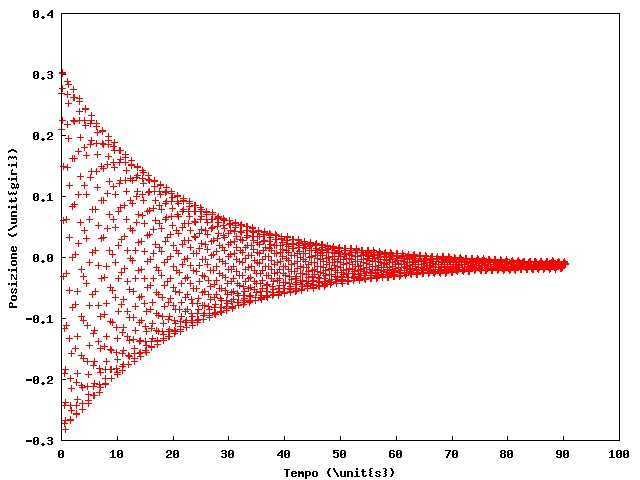
\includegraphics[width = .7\textwidth,angle=-90]{smorz.eps}
% \end{figure}
% \begin{figure}[p]\caption{Fase di smorzamento della durata di 90 secondi, a partire dalla frequenza di risonanza. Le barre di errore sono più piccole delle dimensioni dei punti su questa scala.}\label{smorza}
% \centering
% \includegraphics[width = .7\textwidth,angle=-90]{smorza.eps}
% \end{figure}
% \begin{figure}[p]\caption{Logaritmi dei massimi per la prima serie di dati nella fase di smorzamento. Le barre di errore sono più piccole delle dimensioni dei punti su questa scala.}\label{massimismorz}
% \centering
% % GNUPLOT: LaTeX picture using PSTRICKS macros
% Define new PST objects, if not already defined
\ifx\PSTloaded\undefined
\def\PSTloaded{t}
\psset{arrowsize=.01 3.2 1.4 .3}
\psset{dotsize=.01}
\catcode`@=11

\newpsobject{PST@Border}{psline}{linewidth=.0015,linestyle=solid}
\newpsobject{PST@Axes}{psline}{linewidth=.0015,linestyle=dotted,dotsep=.004}
\newpsobject{PST@Solid}{psline}{linewidth=.0015,linestyle=solid}
\newpsobject{PST@Dashed}{psline}{linewidth=.0015,linestyle=dashed,dash=.01 .01}
\newpsobject{PST@Dotted}{psline}{linewidth=.0025,linestyle=dotted,dotsep=.008}
\newpsobject{PST@LongDash}{psline}{linewidth=.0015,linestyle=dashed,dash=.02 .01}
\newpsobject{PST@Diamond}{psdots}{linewidth=.001,linestyle=solid,dotstyle=square,dotangle=45}
\newpsobject{PST@Filldiamond}{psdots}{linewidth=.001,linestyle=solid,dotstyle=square*,dotangle=45}
\newpsobject{PST@Cross}{psdots}{linewidth=.001,linestyle=solid,dotstyle=+,dotangle=45}
\newpsobject{PST@Plus}{psdots}{linewidth=.001,linestyle=solid,dotstyle=+}
\newpsobject{PST@Square}{psdots}{linewidth=.001,linestyle=solid,dotstyle=square}
\newpsobject{PST@Circle}{psdots}{linewidth=.001,linestyle=solid,dotstyle=o}
\newpsobject{PST@Triangle}{psdots}{linewidth=.001,linestyle=solid,dotstyle=triangle}
\newpsobject{PST@Pentagon}{psdots}{linewidth=.001,linestyle=solid,dotstyle=pentagon}
\newpsobject{PST@Fillsquare}{psdots}{linewidth=.001,linestyle=solid,dotstyle=square*}
\newpsobject{PST@Fillcircle}{psdots}{linewidth=.001,linestyle=solid,dotstyle=*}
\newpsobject{PST@Filltriangle}{psdots}{linewidth=.001,linestyle=solid,dotstyle=triangle*}
\newpsobject{PST@Fillpentagon}{psdots}{linewidth=.001,linestyle=solid,dotstyle=pentagon*}
\newpsobject{PST@Arrow}{psline}{linewidth=.001,linestyle=solid}
\catcode`@=12

\fi
\psset{unit=5.0in,xunit=5.0in,yunit=3.0in}
\pspicture(0.000000,0.000000)(1.000000,1.000000)
\ifx\nofigs\undefined
\catcode`@=11

\PST@Border(0.1590,0.1260)
(0.1740,0.1260)

\rput[r](0.1430,0.1260){-5.5}
\PST@Border(0.1590,0.2944)
(0.1740,0.2944)

\rput[r](0.1430,0.2944){-5.0}
\PST@Border(0.1590,0.4628)
(0.1740,0.4628)

\rput[r](0.1430,0.4628){-4.5}
\PST@Border(0.1590,0.6312)
(0.1740,0.6312)

\rput[r](0.1430,0.6312){-4.0}
\PST@Border(0.1590,0.7996)
(0.1740,0.7996)

\rput[r](0.1430,0.7996){-3.5}
\PST@Border(0.1590,0.9680)
(0.1740,0.9680)

\rput[r](0.1430,0.9680){-3.0}
\PST@Border(0.1590,0.1260)
(0.1590,0.1460)

\rput(0.1590,0.0840){0}
\PST@Border(0.2575,0.1260)
(0.2575,0.1460)

\rput(0.2575,0.0840){5}
\PST@Border(0.3560,0.1260)
(0.3560,0.1460)

\rput(0.3560,0.0840){10}
\PST@Border(0.4545,0.1260)
(0.4545,0.1460)

\rput(0.4545,0.0840){15}
\PST@Border(0.5530,0.1260)
(0.5530,0.1460)

\rput(0.5530,0.0840){20}
\PST@Border(0.6515,0.1260)
(0.6515,0.1460)

\rput(0.6515,0.0840){25}
\PST@Border(0.7500,0.1260)
(0.7500,0.1460)

\rput(0.7500,0.0840){30}
\PST@Border(0.8485,0.1260)
(0.8485,0.1460)

\rput(0.8485,0.0840){35}
\PST@Border(0.9470,0.1260)
(0.9470,0.1460)

\rput(0.9470,0.0840){40}
\PST@Border(0.1590,0.9680)
(0.1590,0.1260)
(0.9470,0.1260)
(0.9470,0.9680)
(0.1590,0.9680)

\rput{L}(0.0420,0.5470){Posizione (\unit{giri})}
\rput(0.5530,0.0210){Tempo (\unit{s})}
\PST@Diamond(0.1620,0.9584)
\PST@Diamond(0.1620,0.9584)
\PST@Diamond(0.1817,0.9413)
\PST@Diamond(0.1620,0.9584)
\PST@Diamond(0.1817,0.9413)
\PST@Diamond(0.2023,0.9258)
\PST@Diamond(0.1620,0.9584)
\PST@Diamond(0.1817,0.9413)
\PST@Diamond(0.2023,0.9258)
\PST@Diamond(0.2230,0.9057)
\PST@Diamond(0.1620,0.9584)
\PST@Diamond(0.1817,0.9413)
\PST@Diamond(0.2023,0.9258)
\PST@Diamond(0.2230,0.9057)
\PST@Diamond(0.2427,0.8843)
\PST@Diamond(0.1620,0.9584)
\PST@Diamond(0.1817,0.9413)
\PST@Diamond(0.2023,0.9258)
\PST@Diamond(0.2230,0.9057)
\PST@Diamond(0.2427,0.8843)
\PST@Diamond(0.2634,0.8688)
\PST@Diamond(0.1620,0.9584)
\PST@Diamond(0.1817,0.9413)
\PST@Diamond(0.2023,0.9258)
\PST@Diamond(0.2230,0.9057)
\PST@Diamond(0.2427,0.8843)
\PST@Diamond(0.2634,0.8688)
\PST@Diamond(0.2841,0.8494)
\PST@Diamond(0.1620,0.9584)
\PST@Diamond(0.1817,0.9413)
\PST@Diamond(0.2023,0.9258)
\PST@Diamond(0.2230,0.9057)
\PST@Diamond(0.2427,0.8843)
\PST@Diamond(0.2634,0.8688)
\PST@Diamond(0.2841,0.8494)
\PST@Diamond(0.3038,0.8306)
\PST@Diamond(0.1620,0.9584)
\PST@Diamond(0.1817,0.9413)
\PST@Diamond(0.2023,0.9258)
\PST@Diamond(0.2230,0.9057)
\PST@Diamond(0.2427,0.8843)
\PST@Diamond(0.2634,0.8688)
\PST@Diamond(0.2841,0.8494)
\PST@Diamond(0.3038,0.8306)
\PST@Diamond(0.3245,0.8140)
\PST@Diamond(0.1620,0.9584)
\PST@Diamond(0.1817,0.9413)
\PST@Diamond(0.2023,0.9258)
\PST@Diamond(0.2230,0.9057)
\PST@Diamond(0.2427,0.8843)
\PST@Diamond(0.2634,0.8688)
\PST@Diamond(0.2841,0.8494)
\PST@Diamond(0.3038,0.8306)
\PST@Diamond(0.3245,0.8140)
\PST@Diamond(0.3452,0.7965)
\PST@Diamond(0.1620,0.9584)
\PST@Diamond(0.1817,0.9413)
\PST@Diamond(0.2023,0.9258)
\PST@Diamond(0.2230,0.9057)
\PST@Diamond(0.2427,0.8843)
\PST@Diamond(0.2634,0.8688)
\PST@Diamond(0.2841,0.8494)
\PST@Diamond(0.3038,0.8306)
\PST@Diamond(0.3245,0.8140)
\PST@Diamond(0.3452,0.7965)
\PST@Diamond(0.3856,0.7606)
\PST@Diamond(0.1620,0.9584)
\PST@Diamond(0.1817,0.9413)
\PST@Diamond(0.2023,0.9258)
\PST@Diamond(0.2230,0.9057)
\PST@Diamond(0.2427,0.8843)
\PST@Diamond(0.2634,0.8688)
\PST@Diamond(0.2841,0.8494)
\PST@Diamond(0.3038,0.8306)
\PST@Diamond(0.3245,0.8140)
\PST@Diamond(0.3452,0.7965)
\PST@Diamond(0.3856,0.7606)
\PST@Diamond(0.4062,0.7401)
\PST@Diamond(0.1620,0.9584)
\PST@Diamond(0.1817,0.9413)
\PST@Diamond(0.2023,0.9258)
\PST@Diamond(0.2230,0.9057)
\PST@Diamond(0.2427,0.8843)
\PST@Diamond(0.2634,0.8688)
\PST@Diamond(0.2841,0.8494)
\PST@Diamond(0.3038,0.8306)
\PST@Diamond(0.3245,0.8140)
\PST@Diamond(0.3452,0.7965)
\PST@Diamond(0.3856,0.7606)
\PST@Diamond(0.4062,0.7401)
\PST@Diamond(0.4269,0.7182)
\PST@Diamond(0.1620,0.9584)
\PST@Diamond(0.1817,0.9413)
\PST@Diamond(0.2023,0.9258)
\PST@Diamond(0.2230,0.9057)
\PST@Diamond(0.2427,0.8843)
\PST@Diamond(0.2634,0.8688)
\PST@Diamond(0.2841,0.8494)
\PST@Diamond(0.3038,0.8306)
\PST@Diamond(0.3245,0.8140)
\PST@Diamond(0.3452,0.7965)
\PST@Diamond(0.3856,0.7606)
\PST@Diamond(0.4062,0.7401)
\PST@Diamond(0.4269,0.7182)
\PST@Diamond(0.4466,0.7020)
\PST@Diamond(0.1620,0.9584)
\PST@Diamond(0.1817,0.9413)
\PST@Diamond(0.2023,0.9258)
\PST@Diamond(0.2230,0.9057)
\PST@Diamond(0.2427,0.8843)
\PST@Diamond(0.2634,0.8688)
\PST@Diamond(0.2841,0.8494)
\PST@Diamond(0.3038,0.8306)
\PST@Diamond(0.3245,0.8140)
\PST@Diamond(0.3452,0.7965)
\PST@Diamond(0.3856,0.7606)
\PST@Diamond(0.4062,0.7401)
\PST@Diamond(0.4269,0.7182)
\PST@Diamond(0.4466,0.7020)
\PST@Diamond(0.4673,0.6825)
\PST@Diamond(0.1620,0.9584)
\PST@Diamond(0.1817,0.9413)
\PST@Diamond(0.2023,0.9258)
\PST@Diamond(0.2230,0.9057)
\PST@Diamond(0.2427,0.8843)
\PST@Diamond(0.2634,0.8688)
\PST@Diamond(0.2841,0.8494)
\PST@Diamond(0.3038,0.8306)
\PST@Diamond(0.3245,0.8140)
\PST@Diamond(0.3452,0.7965)
\PST@Diamond(0.3856,0.7606)
\PST@Diamond(0.4062,0.7401)
\PST@Diamond(0.4269,0.7182)
\PST@Diamond(0.4466,0.7020)
\PST@Diamond(0.4673,0.6825)
\PST@Diamond(0.4880,0.6644)
\PST@Diamond(0.1620,0.9584)
\PST@Diamond(0.1817,0.9413)
\PST@Diamond(0.2023,0.9258)
\PST@Diamond(0.2230,0.9057)
\PST@Diamond(0.2427,0.8843)
\PST@Diamond(0.2634,0.8688)
\PST@Diamond(0.2841,0.8494)
\PST@Diamond(0.3038,0.8306)
\PST@Diamond(0.3245,0.8140)
\PST@Diamond(0.3452,0.7965)
\PST@Diamond(0.3856,0.7606)
\PST@Diamond(0.4062,0.7401)
\PST@Diamond(0.4269,0.7182)
\PST@Diamond(0.4466,0.7020)
\PST@Diamond(0.4673,0.6825)
\PST@Diamond(0.4880,0.6644)
\PST@Diamond(0.5077,0.6453)
\PST@Diamond(0.1620,0.9584)
\PST@Diamond(0.1817,0.9413)
\PST@Diamond(0.2023,0.9258)
\PST@Diamond(0.2230,0.9057)
\PST@Diamond(0.2427,0.8843)
\PST@Diamond(0.2634,0.8688)
\PST@Diamond(0.2841,0.8494)
\PST@Diamond(0.3038,0.8306)
\PST@Diamond(0.3245,0.8140)
\PST@Diamond(0.3452,0.7965)
\PST@Diamond(0.3856,0.7606)
\PST@Diamond(0.4062,0.7401)
\PST@Diamond(0.4269,0.7182)
\PST@Diamond(0.4466,0.7020)
\PST@Diamond(0.4673,0.6825)
\PST@Diamond(0.4880,0.6644)
\PST@Diamond(0.5077,0.6453)
\PST@Diamond(0.5284,0.6280)
\PST@Diamond(0.1620,0.9584)
\PST@Diamond(0.1817,0.9413)
\PST@Diamond(0.2023,0.9258)
\PST@Diamond(0.2230,0.9057)
\PST@Diamond(0.2427,0.8843)
\PST@Diamond(0.2634,0.8688)
\PST@Diamond(0.2841,0.8494)
\PST@Diamond(0.3038,0.8306)
\PST@Diamond(0.3245,0.8140)
\PST@Diamond(0.3452,0.7965)
\PST@Diamond(0.3856,0.7606)
\PST@Diamond(0.4062,0.7401)
\PST@Diamond(0.4269,0.7182)
\PST@Diamond(0.4466,0.7020)
\PST@Diamond(0.4673,0.6825)
\PST@Diamond(0.4880,0.6644)
\PST@Diamond(0.5077,0.6453)
\PST@Diamond(0.5284,0.6280)
\PST@Diamond(0.5491,0.6098)
\PST@Diamond(0.1620,0.9584)
\PST@Diamond(0.1817,0.9413)
\PST@Diamond(0.2023,0.9258)
\PST@Diamond(0.2230,0.9057)
\PST@Diamond(0.2427,0.8843)
\PST@Diamond(0.2634,0.8688)
\PST@Diamond(0.2841,0.8494)
\PST@Diamond(0.3038,0.8306)
\PST@Diamond(0.3245,0.8140)
\PST@Diamond(0.3452,0.7965)
\PST@Diamond(0.3856,0.7606)
\PST@Diamond(0.4062,0.7401)
\PST@Diamond(0.4269,0.7182)
\PST@Diamond(0.4466,0.7020)
\PST@Diamond(0.4673,0.6825)
\PST@Diamond(0.4880,0.6644)
\PST@Diamond(0.5077,0.6453)
\PST@Diamond(0.5284,0.6280)
\PST@Diamond(0.5491,0.6098)
\PST@Diamond(0.5688,0.5872)
\PST@Diamond(0.1620,0.9584)
\PST@Diamond(0.1817,0.9413)
\PST@Diamond(0.2023,0.9258)
\PST@Diamond(0.2230,0.9057)
\PST@Diamond(0.2427,0.8843)
\PST@Diamond(0.2634,0.8688)
\PST@Diamond(0.2841,0.8494)
\PST@Diamond(0.3038,0.8306)
\PST@Diamond(0.3245,0.8140)
\PST@Diamond(0.3452,0.7965)
\PST@Diamond(0.3856,0.7606)
\PST@Diamond(0.4062,0.7401)
\PST@Diamond(0.4269,0.7182)
\PST@Diamond(0.4466,0.7020)
\PST@Diamond(0.4673,0.6825)
\PST@Diamond(0.4880,0.6644)
\PST@Diamond(0.5077,0.6453)
\PST@Diamond(0.5284,0.6280)
\PST@Diamond(0.5491,0.6098)
\PST@Diamond(0.5688,0.5872)
\PST@Diamond(0.5894,0.5736)
\PST@Diamond(0.1620,0.9584)
\PST@Diamond(0.1817,0.9413)
\PST@Diamond(0.2023,0.9258)
\PST@Diamond(0.2230,0.9057)
\PST@Diamond(0.2427,0.8843)
\PST@Diamond(0.2634,0.8688)
\PST@Diamond(0.2841,0.8494)
\PST@Diamond(0.3038,0.8306)
\PST@Diamond(0.3245,0.8140)
\PST@Diamond(0.3452,0.7965)
\PST@Diamond(0.3856,0.7606)
\PST@Diamond(0.4062,0.7401)
\PST@Diamond(0.4269,0.7182)
\PST@Diamond(0.4466,0.7020)
\PST@Diamond(0.4673,0.6825)
\PST@Diamond(0.4880,0.6644)
\PST@Diamond(0.5077,0.6453)
\PST@Diamond(0.5284,0.6280)
\PST@Diamond(0.5491,0.6098)
\PST@Diamond(0.5688,0.5872)
\PST@Diamond(0.5894,0.5736)
\PST@Diamond(0.6101,0.5521)
\PST@Diamond(0.1620,0.9584)
\PST@Diamond(0.1817,0.9413)
\PST@Diamond(0.2023,0.9258)
\PST@Diamond(0.2230,0.9057)
\PST@Diamond(0.2427,0.8843)
\PST@Diamond(0.2634,0.8688)
\PST@Diamond(0.2841,0.8494)
\PST@Diamond(0.3038,0.8306)
\PST@Diamond(0.3245,0.8140)
\PST@Diamond(0.3452,0.7965)
\PST@Diamond(0.3856,0.7606)
\PST@Diamond(0.4062,0.7401)
\PST@Diamond(0.4269,0.7182)
\PST@Diamond(0.4466,0.7020)
\PST@Diamond(0.4673,0.6825)
\PST@Diamond(0.4880,0.6644)
\PST@Diamond(0.5077,0.6453)
\PST@Diamond(0.5284,0.6280)
\PST@Diamond(0.5491,0.6098)
\PST@Diamond(0.5688,0.5872)
\PST@Diamond(0.5894,0.5736)
\PST@Diamond(0.6101,0.5521)
\PST@Diamond(0.6505,0.5171)
\PST@Diamond(0.1620,0.9584)
\PST@Diamond(0.1817,0.9413)
\PST@Diamond(0.2023,0.9258)
\PST@Diamond(0.2230,0.9057)
\PST@Diamond(0.2427,0.8843)
\PST@Diamond(0.2634,0.8688)
\PST@Diamond(0.2841,0.8494)
\PST@Diamond(0.3038,0.8306)
\PST@Diamond(0.3245,0.8140)
\PST@Diamond(0.3452,0.7965)
\PST@Diamond(0.3856,0.7606)
\PST@Diamond(0.4062,0.7401)
\PST@Diamond(0.4269,0.7182)
\PST@Diamond(0.4466,0.7020)
\PST@Diamond(0.4673,0.6825)
\PST@Diamond(0.4880,0.6644)
\PST@Diamond(0.5077,0.6453)
\PST@Diamond(0.5284,0.6280)
\PST@Diamond(0.5491,0.6098)
\PST@Diamond(0.5688,0.5872)
\PST@Diamond(0.5894,0.5736)
\PST@Diamond(0.6101,0.5521)
\PST@Diamond(0.6505,0.5171)
\PST@Diamond(0.6712,0.4915)
\PST@Diamond(0.1620,0.9584)
\PST@Diamond(0.1817,0.9413)
\PST@Diamond(0.2023,0.9258)
\PST@Diamond(0.2230,0.9057)
\PST@Diamond(0.2427,0.8843)
\PST@Diamond(0.2634,0.8688)
\PST@Diamond(0.2841,0.8494)
\PST@Diamond(0.3038,0.8306)
\PST@Diamond(0.3245,0.8140)
\PST@Diamond(0.3452,0.7965)
\PST@Diamond(0.3856,0.7606)
\PST@Diamond(0.4062,0.7401)
\PST@Diamond(0.4269,0.7182)
\PST@Diamond(0.4466,0.7020)
\PST@Diamond(0.4673,0.6825)
\PST@Diamond(0.4880,0.6644)
\PST@Diamond(0.5077,0.6453)
\PST@Diamond(0.5284,0.6280)
\PST@Diamond(0.5491,0.6098)
\PST@Diamond(0.5688,0.5872)
\PST@Diamond(0.5894,0.5736)
\PST@Diamond(0.6101,0.5521)
\PST@Diamond(0.6505,0.5171)
\PST@Diamond(0.6712,0.4915)
\PST@Diamond(0.6919,0.4779)
\PST@Diamond(0.1620,0.9584)
\PST@Diamond(0.1817,0.9413)
\PST@Diamond(0.2023,0.9258)
\PST@Diamond(0.2230,0.9057)
\PST@Diamond(0.2427,0.8843)
\PST@Diamond(0.2634,0.8688)
\PST@Diamond(0.2841,0.8494)
\PST@Diamond(0.3038,0.8306)
\PST@Diamond(0.3245,0.8140)
\PST@Diamond(0.3452,0.7965)
\PST@Diamond(0.3856,0.7606)
\PST@Diamond(0.4062,0.7401)
\PST@Diamond(0.4269,0.7182)
\PST@Diamond(0.4466,0.7020)
\PST@Diamond(0.4673,0.6825)
\PST@Diamond(0.4880,0.6644)
\PST@Diamond(0.5077,0.6453)
\PST@Diamond(0.5284,0.6280)
\PST@Diamond(0.5491,0.6098)
\PST@Diamond(0.5688,0.5872)
\PST@Diamond(0.5894,0.5736)
\PST@Diamond(0.6101,0.5521)
\PST@Diamond(0.6505,0.5171)
\PST@Diamond(0.6712,0.4915)
\PST@Diamond(0.6919,0.4779)
\PST@Diamond(0.7116,0.4540)
\PST@Diamond(0.1620,0.9584)
\PST@Diamond(0.1817,0.9413)
\PST@Diamond(0.2023,0.9258)
\PST@Diamond(0.2230,0.9057)
\PST@Diamond(0.2427,0.8843)
\PST@Diamond(0.2634,0.8688)
\PST@Diamond(0.2841,0.8494)
\PST@Diamond(0.3038,0.8306)
\PST@Diamond(0.3245,0.8140)
\PST@Diamond(0.3452,0.7965)
\PST@Diamond(0.3856,0.7606)
\PST@Diamond(0.4062,0.7401)
\PST@Diamond(0.4269,0.7182)
\PST@Diamond(0.4466,0.7020)
\PST@Diamond(0.4673,0.6825)
\PST@Diamond(0.4880,0.6644)
\PST@Diamond(0.5077,0.6453)
\PST@Diamond(0.5284,0.6280)
\PST@Diamond(0.5491,0.6098)
\PST@Diamond(0.5688,0.5872)
\PST@Diamond(0.5894,0.5736)
\PST@Diamond(0.6101,0.5521)
\PST@Diamond(0.6505,0.5171)
\PST@Diamond(0.6712,0.4915)
\PST@Diamond(0.6919,0.4779)
\PST@Diamond(0.7116,0.4540)
\PST@Diamond(0.7323,0.4336)
\PST@Diamond(0.1620,0.9584)
\PST@Diamond(0.1817,0.9413)
\PST@Diamond(0.2023,0.9258)
\PST@Diamond(0.2230,0.9057)
\PST@Diamond(0.2427,0.8843)
\PST@Diamond(0.2634,0.8688)
\PST@Diamond(0.2841,0.8494)
\PST@Diamond(0.3038,0.8306)
\PST@Diamond(0.3245,0.8140)
\PST@Diamond(0.3452,0.7965)
\PST@Diamond(0.3856,0.7606)
\PST@Diamond(0.4062,0.7401)
\PST@Diamond(0.4269,0.7182)
\PST@Diamond(0.4466,0.7020)
\PST@Diamond(0.4673,0.6825)
\PST@Diamond(0.4880,0.6644)
\PST@Diamond(0.5077,0.6453)
\PST@Diamond(0.5284,0.6280)
\PST@Diamond(0.5491,0.6098)
\PST@Diamond(0.5688,0.5872)
\PST@Diamond(0.5894,0.5736)
\PST@Diamond(0.6101,0.5521)
\PST@Diamond(0.6505,0.5171)
\PST@Diamond(0.6712,0.4915)
\PST@Diamond(0.6919,0.4779)
\PST@Diamond(0.7116,0.4540)
\PST@Diamond(0.7323,0.4336)
\PST@Diamond(0.7727,0.4004)
\PST@Diamond(0.1620,0.9584)
\PST@Diamond(0.1817,0.9413)
\PST@Diamond(0.2023,0.9258)
\PST@Diamond(0.2230,0.9057)
\PST@Diamond(0.2427,0.8843)
\PST@Diamond(0.2634,0.8688)
\PST@Diamond(0.2841,0.8494)
\PST@Diamond(0.3038,0.8306)
\PST@Diamond(0.3245,0.8140)
\PST@Diamond(0.3452,0.7965)
\PST@Diamond(0.3856,0.7606)
\PST@Diamond(0.4062,0.7401)
\PST@Diamond(0.4269,0.7182)
\PST@Diamond(0.4466,0.7020)
\PST@Diamond(0.4673,0.6825)
\PST@Diamond(0.4880,0.6644)
\PST@Diamond(0.5077,0.6453)
\PST@Diamond(0.5284,0.6280)
\PST@Diamond(0.5491,0.6098)
\PST@Diamond(0.5688,0.5872)
\PST@Diamond(0.5894,0.5736)
\PST@Diamond(0.6101,0.5521)
\PST@Diamond(0.6505,0.5171)
\PST@Diamond(0.6712,0.4915)
\PST@Diamond(0.6919,0.4779)
\PST@Diamond(0.7116,0.4540)
\PST@Diamond(0.7323,0.4336)
\PST@Diamond(0.7727,0.4004)
\PST@Diamond(0.7933,0.3764)
\PST@Diamond(0.1620,0.9584)
\PST@Diamond(0.1817,0.9413)
\PST@Diamond(0.2023,0.9258)
\PST@Diamond(0.2230,0.9057)
\PST@Diamond(0.2427,0.8843)
\PST@Diamond(0.2634,0.8688)
\PST@Diamond(0.2841,0.8494)
\PST@Diamond(0.3038,0.8306)
\PST@Diamond(0.3245,0.8140)
\PST@Diamond(0.3452,0.7965)
\PST@Diamond(0.3856,0.7606)
\PST@Diamond(0.4062,0.7401)
\PST@Diamond(0.4269,0.7182)
\PST@Diamond(0.4466,0.7020)
\PST@Diamond(0.4673,0.6825)
\PST@Diamond(0.4880,0.6644)
\PST@Diamond(0.5077,0.6453)
\PST@Diamond(0.5284,0.6280)
\PST@Diamond(0.5491,0.6098)
\PST@Diamond(0.5688,0.5872)
\PST@Diamond(0.5894,0.5736)
\PST@Diamond(0.6101,0.5521)
\PST@Diamond(0.6505,0.5171)
\PST@Diamond(0.6712,0.4915)
\PST@Diamond(0.6919,0.4779)
\PST@Diamond(0.7116,0.4540)
\PST@Diamond(0.7323,0.4336)
\PST@Diamond(0.7727,0.4004)
\PST@Diamond(0.7933,0.3764)
\PST@Diamond(0.8337,0.3436)
\PST@Diamond(0.1620,0.9584)
\PST@Diamond(0.1817,0.9413)
\PST@Diamond(0.2023,0.9258)
\PST@Diamond(0.2230,0.9057)
\PST@Diamond(0.2427,0.8843)
\PST@Diamond(0.2634,0.8688)
\PST@Diamond(0.2841,0.8494)
\PST@Diamond(0.3038,0.8306)
\PST@Diamond(0.3245,0.8140)
\PST@Diamond(0.3452,0.7965)
\PST@Diamond(0.3856,0.7606)
\PST@Diamond(0.4062,0.7401)
\PST@Diamond(0.4269,0.7182)
\PST@Diamond(0.4466,0.7020)
\PST@Diamond(0.4673,0.6825)
\PST@Diamond(0.4880,0.6644)
\PST@Diamond(0.5077,0.6453)
\PST@Diamond(0.5284,0.6280)
\PST@Diamond(0.5491,0.6098)
\PST@Diamond(0.5688,0.5872)
\PST@Diamond(0.5894,0.5736)
\PST@Diamond(0.6101,0.5521)
\PST@Diamond(0.6505,0.5171)
\PST@Diamond(0.6712,0.4915)
\PST@Diamond(0.6919,0.4779)
\PST@Diamond(0.7116,0.4540)
\PST@Diamond(0.7323,0.4336)
\PST@Diamond(0.7727,0.4004)
\PST@Diamond(0.7933,0.3764)
\PST@Diamond(0.8337,0.3436)
\PST@Diamond(0.8544,0.3150)
\PST@Diamond(0.1620,0.9584)
\PST@Diamond(0.1817,0.9413)
\PST@Diamond(0.2023,0.9258)
\PST@Diamond(0.2230,0.9057)
\PST@Diamond(0.2427,0.8843)
\PST@Diamond(0.2634,0.8688)
\PST@Diamond(0.2841,0.8494)
\PST@Diamond(0.3038,0.8306)
\PST@Diamond(0.3245,0.8140)
\PST@Diamond(0.3452,0.7965)
\PST@Diamond(0.3856,0.7606)
\PST@Diamond(0.4062,0.7401)
\PST@Diamond(0.4269,0.7182)
\PST@Diamond(0.4466,0.7020)
\PST@Diamond(0.4673,0.6825)
\PST@Diamond(0.4880,0.6644)
\PST@Diamond(0.5077,0.6453)
\PST@Diamond(0.5284,0.6280)
\PST@Diamond(0.5491,0.6098)
\PST@Diamond(0.5688,0.5872)
\PST@Diamond(0.5894,0.5736)
\PST@Diamond(0.6101,0.5521)
\PST@Diamond(0.6505,0.5171)
\PST@Diamond(0.6712,0.4915)
\PST@Diamond(0.6919,0.4779)
\PST@Diamond(0.7116,0.4540)
\PST@Diamond(0.7323,0.4336)
\PST@Diamond(0.7727,0.4004)
\PST@Diamond(0.7933,0.3764)
\PST@Diamond(0.8337,0.3436)
\PST@Diamond(0.8544,0.3150)
\PST@Diamond(0.8751,0.2996)
\PST@Diamond(0.1620,0.9584)
\PST@Diamond(0.1817,0.9413)
\PST@Diamond(0.2023,0.9258)
\PST@Diamond(0.2230,0.9057)
\PST@Diamond(0.2427,0.8843)
\PST@Diamond(0.2634,0.8688)
\PST@Diamond(0.2841,0.8494)
\PST@Diamond(0.3038,0.8306)
\PST@Diamond(0.3245,0.8140)
\PST@Diamond(0.3452,0.7965)
\PST@Diamond(0.3856,0.7606)
\PST@Diamond(0.4062,0.7401)
\PST@Diamond(0.4269,0.7182)
\PST@Diamond(0.4466,0.7020)
\PST@Diamond(0.4673,0.6825)
\PST@Diamond(0.4880,0.6644)
\PST@Diamond(0.5077,0.6453)
\PST@Diamond(0.5284,0.6280)
\PST@Diamond(0.5491,0.6098)
\PST@Diamond(0.5688,0.5872)
\PST@Diamond(0.5894,0.5736)
\PST@Diamond(0.6101,0.5521)
\PST@Diamond(0.6505,0.5171)
\PST@Diamond(0.6712,0.4915)
\PST@Diamond(0.6919,0.4779)
\PST@Diamond(0.7116,0.4540)
\PST@Diamond(0.7323,0.4336)
\PST@Diamond(0.7727,0.4004)
\PST@Diamond(0.7933,0.3764)
\PST@Diamond(0.8337,0.3436)
\PST@Diamond(0.8544,0.3150)
\PST@Diamond(0.8751,0.2996)
\PST@Diamond(0.8948,0.2753)
\PST@Diamond(0.1620,0.9584)
\PST@Diamond(0.1817,0.9413)
\PST@Diamond(0.2023,0.9258)
\PST@Diamond(0.2230,0.9057)
\PST@Diamond(0.2427,0.8843)
\PST@Diamond(0.2634,0.8688)
\PST@Diamond(0.2841,0.8494)
\PST@Diamond(0.3038,0.8306)
\PST@Diamond(0.3245,0.8140)
\PST@Diamond(0.3452,0.7965)
\PST@Diamond(0.3856,0.7606)
\PST@Diamond(0.4062,0.7401)
\PST@Diamond(0.4269,0.7182)
\PST@Diamond(0.4466,0.7020)
\PST@Diamond(0.4673,0.6825)
\PST@Diamond(0.4880,0.6644)
\PST@Diamond(0.5077,0.6453)
\PST@Diamond(0.5284,0.6280)
\PST@Diamond(0.5491,0.6098)
\PST@Diamond(0.5688,0.5872)
\PST@Diamond(0.5894,0.5736)
\PST@Diamond(0.6101,0.5521)
\PST@Diamond(0.6505,0.5171)
\PST@Diamond(0.6712,0.4915)
\PST@Diamond(0.6919,0.4779)
\PST@Diamond(0.7116,0.4540)
\PST@Diamond(0.7323,0.4336)
\PST@Diamond(0.7727,0.4004)
\PST@Diamond(0.7933,0.3764)
\PST@Diamond(0.8337,0.3436)
\PST@Diamond(0.8544,0.3150)
\PST@Diamond(0.8751,0.2996)
\PST@Diamond(0.8948,0.2753)
\PST@Diamond(0.9362,0.2303)
\PST@Dashed(0.1620,0.9649)
(0.1620,0.9649)
(0.1698,0.9576)
(0.1776,0.9503)
(0.1854,0.9431)
(0.1932,0.9358)
(0.2011,0.9285)
(0.2089,0.9212)
(0.2167,0.9140)
(0.2245,0.9067)
(0.2323,0.8994)
(0.2402,0.8921)
(0.2480,0.8849)
(0.2558,0.8776)
(0.2636,0.8703)
(0.2714,0.8630)
(0.2793,0.8558)
(0.2871,0.8485)
(0.2949,0.8412)
(0.3027,0.8339)
(0.3105,0.8267)
(0.3184,0.8194)
(0.3262,0.8121)
(0.3340,0.8048)
(0.3418,0.7976)
(0.3496,0.7903)
(0.3575,0.7830)
(0.3653,0.7757)
(0.3731,0.7685)
(0.3809,0.7612)
(0.3887,0.7539)
(0.3966,0.7466)
(0.4044,0.7393)
(0.4122,0.7321)
(0.4200,0.7248)
(0.4278,0.7175)
(0.4357,0.7102)
(0.4435,0.7030)
(0.4513,0.6957)
(0.4591,0.6884)
(0.4669,0.6811)
(0.4748,0.6739)
(0.4826,0.6666)
(0.4904,0.6593)
(0.4982,0.6520)
(0.5060,0.6448)
(0.5139,0.6375)
(0.5217,0.6302)
(0.5295,0.6229)
(0.5373,0.6157)
(0.5451,0.6084)
(0.5530,0.6011)
(0.5608,0.5938)
(0.5686,0.5866)
(0.5764,0.5793)
(0.5843,0.5720)
(0.5921,0.5647)
(0.5999,0.5575)
(0.6077,0.5502)
(0.6155,0.5429)
(0.6234,0.5356)
(0.6312,0.5284)
(0.6390,0.5211)
(0.6468,0.5138)
(0.6546,0.5065)
(0.6625,0.4992)
(0.6703,0.4920)
(0.6781,0.4847)
(0.6859,0.4774)
(0.6937,0.4701)
(0.7016,0.4629)
(0.7094,0.4556)
(0.7172,0.4483)
(0.7250,0.4410)
(0.7328,0.4338)
(0.7407,0.4265)
(0.7485,0.4192)
(0.7563,0.4119)
(0.7641,0.4047)
(0.7719,0.3974)
(0.7798,0.3901)
(0.7876,0.3828)
(0.7954,0.3756)
(0.8032,0.3683)
(0.8110,0.3610)
(0.8189,0.3537)
(0.8267,0.3465)
(0.8345,0.3392)
(0.8423,0.3319)
(0.8501,0.3246)
(0.8580,0.3174)
(0.8658,0.3101)
(0.8736,0.3028)
(0.8814,0.2955)
(0.8892,0.2883)
(0.8971,0.2810)
(0.9049,0.2737)
(0.9127,0.2664)
(0.9205,0.2592)
(0.9283,0.2519)
(0.9362,0.2446)

\PST@Border(0.1590,0.9680)
(0.1590,0.1260)
(0.9470,0.1260)
(0.9470,0.9680)
(0.1590,0.9680)

\catcode`@=12
\fi
\endpspicture

% \end{figure}
% \begin{figure}[p]\caption{Logaritmi dei minimi per la prima serie di dati nella fase di smorzamento. Le barre di errore sono più piccole delle dimensioni dei punti su questa scala.}\label{minimismorz}
% \centering
% % GNUPLOT: LaTeX picture using PSTRICKS macros
% Define new PST objects, if not already defined
\ifx\PSTloaded\undefined
\def\PSTloaded{t}
\psset{arrowsize=.01 3.2 1.4 .3}
\psset{dotsize=.01}
\catcode`@=11

\newpsobject{PST@Border}{psline}{linewidth=.0015,linestyle=solid}
\newpsobject{PST@Axes}{psline}{linewidth=.0015,linestyle=dotted,dotsep=.004}
\newpsobject{PST@Solid}{psline}{linewidth=.0015,linestyle=solid}
\newpsobject{PST@Dashed}{psline}{linewidth=.0015,linestyle=dashed,dash=.01 .01}
\newpsobject{PST@Dotted}{psline}{linewidth=.0025,linestyle=dotted,dotsep=.008}
\newpsobject{PST@LongDash}{psline}{linewidth=.0015,linestyle=dashed,dash=.02 .01}
\newpsobject{PST@Diamond}{psdots}{linewidth=.001,linestyle=solid,dotstyle=square,dotangle=45}
\newpsobject{PST@Filldiamond}{psdots}{linewidth=.001,linestyle=solid,dotstyle=square*,dotangle=45}
\newpsobject{PST@Cross}{psdots}{linewidth=.001,linestyle=solid,dotstyle=+,dotangle=45}
\newpsobject{PST@Plus}{psdots}{linewidth=.001,linestyle=solid,dotstyle=+}
\newpsobject{PST@Square}{psdots}{linewidth=.001,linestyle=solid,dotstyle=square}
\newpsobject{PST@Circle}{psdots}{linewidth=.001,linestyle=solid,dotstyle=o}
\newpsobject{PST@Triangle}{psdots}{linewidth=.001,linestyle=solid,dotstyle=triangle}
\newpsobject{PST@Pentagon}{psdots}{linewidth=.001,linestyle=solid,dotstyle=pentagon}
\newpsobject{PST@Fillsquare}{psdots}{linewidth=.001,linestyle=solid,dotstyle=square*}
\newpsobject{PST@Fillcircle}{psdots}{linewidth=.001,linestyle=solid,dotstyle=*}
\newpsobject{PST@Filltriangle}{psdots}{linewidth=.001,linestyle=solid,dotstyle=triangle*}
\newpsobject{PST@Fillpentagon}{psdots}{linewidth=.001,linestyle=solid,dotstyle=pentagon*}
\newpsobject{PST@Arrow}{psline}{linewidth=.001,linestyle=solid}
\catcode`@=12

\fi
\psset{unit=5.0in,xunit=5.0in,yunit=3.0in}
\pspicture(0.000000,0.000000)(1.000000,1.000000)
\ifx\nofigs\undefined
\catcode`@=11

\PST@Border(0.1590,0.1260)
(0.1740,0.1260)

\rput[r](0.1430,0.1260){-5.5}
\PST@Border(0.1590,0.2944)
(0.1740,0.2944)

\rput[r](0.1430,0.2944){-5.0}
\PST@Border(0.1590,0.4628)
(0.1740,0.4628)

\rput[r](0.1430,0.4628){-4.5}
\PST@Border(0.1590,0.6312)
(0.1740,0.6312)

\rput[r](0.1430,0.6312){-4.0}
\PST@Border(0.1590,0.7996)
(0.1740,0.7996)

\rput[r](0.1430,0.7996){-3.5}
\PST@Border(0.1590,0.9680)
(0.1740,0.9680)

\rput[r](0.1430,0.9680){-3.0}
\PST@Border(0.1590,0.1260)
(0.1590,0.1460)

\rput(0.1590,0.0840){0}
\PST@Border(0.2575,0.1260)
(0.2575,0.1460)

\rput(0.2575,0.0840){5}
\PST@Border(0.3560,0.1260)
(0.3560,0.1460)

\rput(0.3560,0.0840){10}
\PST@Border(0.4545,0.1260)
(0.4545,0.1460)

\rput(0.4545,0.0840){15}
\PST@Border(0.5530,0.1260)
(0.5530,0.1460)

\rput(0.5530,0.0840){20}
\PST@Border(0.6515,0.1260)
(0.6515,0.1460)

\rput(0.6515,0.0840){25}
\PST@Border(0.7500,0.1260)
(0.7500,0.1460)

\rput(0.7500,0.0840){30}
\PST@Border(0.8485,0.1260)
(0.8485,0.1460)

\rput(0.8485,0.0840){35}
\PST@Border(0.9470,0.1260)
(0.9470,0.1460)

\rput(0.9470,0.0840){40}
\PST@Border(0.1590,0.9680)
(0.1590,0.1260)
(0.9470,0.1260)
(0.9470,0.9680)
(0.1590,0.9680)

\rput{L}(0.0420,0.5470){Posizione (\unit{giri})}
\rput(0.5530,0.0210){Tempo (\unit{s})}
\PST@Diamond(0.1620,0.9584)
\PST@Diamond(0.1620,0.9584)
\PST@Diamond(0.1817,0.9413)
\PST@Diamond(0.1620,0.9584)
\PST@Diamond(0.1817,0.9413)
\PST@Diamond(0.2023,0.9258)
\PST@Diamond(0.1620,0.9584)
\PST@Diamond(0.1817,0.9413)
\PST@Diamond(0.2023,0.9258)
\PST@Diamond(0.2230,0.9057)
\PST@Diamond(0.1620,0.9584)
\PST@Diamond(0.1817,0.9413)
\PST@Diamond(0.2023,0.9258)
\PST@Diamond(0.2230,0.9057)
\PST@Diamond(0.2427,0.8843)
\PST@Diamond(0.1620,0.9584)
\PST@Diamond(0.1817,0.9413)
\PST@Diamond(0.2023,0.9258)
\PST@Diamond(0.2230,0.9057)
\PST@Diamond(0.2427,0.8843)
\PST@Diamond(0.2634,0.8688)
\PST@Diamond(0.1620,0.9584)
\PST@Diamond(0.1817,0.9413)
\PST@Diamond(0.2023,0.9258)
\PST@Diamond(0.2230,0.9057)
\PST@Diamond(0.2427,0.8843)
\PST@Diamond(0.2634,0.8688)
\PST@Diamond(0.2841,0.8494)
\PST@Diamond(0.1620,0.9584)
\PST@Diamond(0.1817,0.9413)
\PST@Diamond(0.2023,0.9258)
\PST@Diamond(0.2230,0.9057)
\PST@Diamond(0.2427,0.8843)
\PST@Diamond(0.2634,0.8688)
\PST@Diamond(0.2841,0.8494)
\PST@Diamond(0.3038,0.8306)
\PST@Diamond(0.1620,0.9584)
\PST@Diamond(0.1817,0.9413)
\PST@Diamond(0.2023,0.9258)
\PST@Diamond(0.2230,0.9057)
\PST@Diamond(0.2427,0.8843)
\PST@Diamond(0.2634,0.8688)
\PST@Diamond(0.2841,0.8494)
\PST@Diamond(0.3038,0.8306)
\PST@Diamond(0.3245,0.8140)
\PST@Diamond(0.1620,0.9584)
\PST@Diamond(0.1817,0.9413)
\PST@Diamond(0.2023,0.9258)
\PST@Diamond(0.2230,0.9057)
\PST@Diamond(0.2427,0.8843)
\PST@Diamond(0.2634,0.8688)
\PST@Diamond(0.2841,0.8494)
\PST@Diamond(0.3038,0.8306)
\PST@Diamond(0.3245,0.8140)
\PST@Diamond(0.3452,0.7965)
\PST@Diamond(0.1620,0.9584)
\PST@Diamond(0.1817,0.9413)
\PST@Diamond(0.2023,0.9258)
\PST@Diamond(0.2230,0.9057)
\PST@Diamond(0.2427,0.8843)
\PST@Diamond(0.2634,0.8688)
\PST@Diamond(0.2841,0.8494)
\PST@Diamond(0.3038,0.8306)
\PST@Diamond(0.3245,0.8140)
\PST@Diamond(0.3452,0.7965)
\PST@Diamond(0.3856,0.7606)
\PST@Diamond(0.1620,0.9584)
\PST@Diamond(0.1817,0.9413)
\PST@Diamond(0.2023,0.9258)
\PST@Diamond(0.2230,0.9057)
\PST@Diamond(0.2427,0.8843)
\PST@Diamond(0.2634,0.8688)
\PST@Diamond(0.2841,0.8494)
\PST@Diamond(0.3038,0.8306)
\PST@Diamond(0.3245,0.8140)
\PST@Diamond(0.3452,0.7965)
\PST@Diamond(0.3856,0.7606)
\PST@Diamond(0.4062,0.7401)
\PST@Diamond(0.1620,0.9584)
\PST@Diamond(0.1817,0.9413)
\PST@Diamond(0.2023,0.9258)
\PST@Diamond(0.2230,0.9057)
\PST@Diamond(0.2427,0.8843)
\PST@Diamond(0.2634,0.8688)
\PST@Diamond(0.2841,0.8494)
\PST@Diamond(0.3038,0.8306)
\PST@Diamond(0.3245,0.8140)
\PST@Diamond(0.3452,0.7965)
\PST@Diamond(0.3856,0.7606)
\PST@Diamond(0.4062,0.7401)
\PST@Diamond(0.4269,0.7182)
\PST@Diamond(0.1620,0.9584)
\PST@Diamond(0.1817,0.9413)
\PST@Diamond(0.2023,0.9258)
\PST@Diamond(0.2230,0.9057)
\PST@Diamond(0.2427,0.8843)
\PST@Diamond(0.2634,0.8688)
\PST@Diamond(0.2841,0.8494)
\PST@Diamond(0.3038,0.8306)
\PST@Diamond(0.3245,0.8140)
\PST@Diamond(0.3452,0.7965)
\PST@Diamond(0.3856,0.7606)
\PST@Diamond(0.4062,0.7401)
\PST@Diamond(0.4269,0.7182)
\PST@Diamond(0.4466,0.7020)
\PST@Diamond(0.1620,0.9584)
\PST@Diamond(0.1817,0.9413)
\PST@Diamond(0.2023,0.9258)
\PST@Diamond(0.2230,0.9057)
\PST@Diamond(0.2427,0.8843)
\PST@Diamond(0.2634,0.8688)
\PST@Diamond(0.2841,0.8494)
\PST@Diamond(0.3038,0.8306)
\PST@Diamond(0.3245,0.8140)
\PST@Diamond(0.3452,0.7965)
\PST@Diamond(0.3856,0.7606)
\PST@Diamond(0.4062,0.7401)
\PST@Diamond(0.4269,0.7182)
\PST@Diamond(0.4466,0.7020)
\PST@Diamond(0.4673,0.6825)
\PST@Diamond(0.1620,0.9584)
\PST@Diamond(0.1817,0.9413)
\PST@Diamond(0.2023,0.9258)
\PST@Diamond(0.2230,0.9057)
\PST@Diamond(0.2427,0.8843)
\PST@Diamond(0.2634,0.8688)
\PST@Diamond(0.2841,0.8494)
\PST@Diamond(0.3038,0.8306)
\PST@Diamond(0.3245,0.8140)
\PST@Diamond(0.3452,0.7965)
\PST@Diamond(0.3856,0.7606)
\PST@Diamond(0.4062,0.7401)
\PST@Diamond(0.4269,0.7182)
\PST@Diamond(0.4466,0.7020)
\PST@Diamond(0.4673,0.6825)
\PST@Diamond(0.4880,0.6644)
\PST@Diamond(0.1620,0.9584)
\PST@Diamond(0.1817,0.9413)
\PST@Diamond(0.2023,0.9258)
\PST@Diamond(0.2230,0.9057)
\PST@Diamond(0.2427,0.8843)
\PST@Diamond(0.2634,0.8688)
\PST@Diamond(0.2841,0.8494)
\PST@Diamond(0.3038,0.8306)
\PST@Diamond(0.3245,0.8140)
\PST@Diamond(0.3452,0.7965)
\PST@Diamond(0.3856,0.7606)
\PST@Diamond(0.4062,0.7401)
\PST@Diamond(0.4269,0.7182)
\PST@Diamond(0.4466,0.7020)
\PST@Diamond(0.4673,0.6825)
\PST@Diamond(0.4880,0.6644)
\PST@Diamond(0.5077,0.6453)
\PST@Diamond(0.1620,0.9584)
\PST@Diamond(0.1817,0.9413)
\PST@Diamond(0.2023,0.9258)
\PST@Diamond(0.2230,0.9057)
\PST@Diamond(0.2427,0.8843)
\PST@Diamond(0.2634,0.8688)
\PST@Diamond(0.2841,0.8494)
\PST@Diamond(0.3038,0.8306)
\PST@Diamond(0.3245,0.8140)
\PST@Diamond(0.3452,0.7965)
\PST@Diamond(0.3856,0.7606)
\PST@Diamond(0.4062,0.7401)
\PST@Diamond(0.4269,0.7182)
\PST@Diamond(0.4466,0.7020)
\PST@Diamond(0.4673,0.6825)
\PST@Diamond(0.4880,0.6644)
\PST@Diamond(0.5077,0.6453)
\PST@Diamond(0.5284,0.6280)
\PST@Diamond(0.1620,0.9584)
\PST@Diamond(0.1817,0.9413)
\PST@Diamond(0.2023,0.9258)
\PST@Diamond(0.2230,0.9057)
\PST@Diamond(0.2427,0.8843)
\PST@Diamond(0.2634,0.8688)
\PST@Diamond(0.2841,0.8494)
\PST@Diamond(0.3038,0.8306)
\PST@Diamond(0.3245,0.8140)
\PST@Diamond(0.3452,0.7965)
\PST@Diamond(0.3856,0.7606)
\PST@Diamond(0.4062,0.7401)
\PST@Diamond(0.4269,0.7182)
\PST@Diamond(0.4466,0.7020)
\PST@Diamond(0.4673,0.6825)
\PST@Diamond(0.4880,0.6644)
\PST@Diamond(0.5077,0.6453)
\PST@Diamond(0.5284,0.6280)
\PST@Diamond(0.5491,0.6098)
\PST@Diamond(0.1620,0.9584)
\PST@Diamond(0.1817,0.9413)
\PST@Diamond(0.2023,0.9258)
\PST@Diamond(0.2230,0.9057)
\PST@Diamond(0.2427,0.8843)
\PST@Diamond(0.2634,0.8688)
\PST@Diamond(0.2841,0.8494)
\PST@Diamond(0.3038,0.8306)
\PST@Diamond(0.3245,0.8140)
\PST@Diamond(0.3452,0.7965)
\PST@Diamond(0.3856,0.7606)
\PST@Diamond(0.4062,0.7401)
\PST@Diamond(0.4269,0.7182)
\PST@Diamond(0.4466,0.7020)
\PST@Diamond(0.4673,0.6825)
\PST@Diamond(0.4880,0.6644)
\PST@Diamond(0.5077,0.6453)
\PST@Diamond(0.5284,0.6280)
\PST@Diamond(0.5491,0.6098)
\PST@Diamond(0.5688,0.5872)
\PST@Diamond(0.1620,0.9584)
\PST@Diamond(0.1817,0.9413)
\PST@Diamond(0.2023,0.9258)
\PST@Diamond(0.2230,0.9057)
\PST@Diamond(0.2427,0.8843)
\PST@Diamond(0.2634,0.8688)
\PST@Diamond(0.2841,0.8494)
\PST@Diamond(0.3038,0.8306)
\PST@Diamond(0.3245,0.8140)
\PST@Diamond(0.3452,0.7965)
\PST@Diamond(0.3856,0.7606)
\PST@Diamond(0.4062,0.7401)
\PST@Diamond(0.4269,0.7182)
\PST@Diamond(0.4466,0.7020)
\PST@Diamond(0.4673,0.6825)
\PST@Diamond(0.4880,0.6644)
\PST@Diamond(0.5077,0.6453)
\PST@Diamond(0.5284,0.6280)
\PST@Diamond(0.5491,0.6098)
\PST@Diamond(0.5688,0.5872)
\PST@Diamond(0.5894,0.5736)
\PST@Diamond(0.1620,0.9584)
\PST@Diamond(0.1817,0.9413)
\PST@Diamond(0.2023,0.9258)
\PST@Diamond(0.2230,0.9057)
\PST@Diamond(0.2427,0.8843)
\PST@Diamond(0.2634,0.8688)
\PST@Diamond(0.2841,0.8494)
\PST@Diamond(0.3038,0.8306)
\PST@Diamond(0.3245,0.8140)
\PST@Diamond(0.3452,0.7965)
\PST@Diamond(0.3856,0.7606)
\PST@Diamond(0.4062,0.7401)
\PST@Diamond(0.4269,0.7182)
\PST@Diamond(0.4466,0.7020)
\PST@Diamond(0.4673,0.6825)
\PST@Diamond(0.4880,0.6644)
\PST@Diamond(0.5077,0.6453)
\PST@Diamond(0.5284,0.6280)
\PST@Diamond(0.5491,0.6098)
\PST@Diamond(0.5688,0.5872)
\PST@Diamond(0.5894,0.5736)
\PST@Diamond(0.6101,0.5521)
\PST@Diamond(0.1620,0.9584)
\PST@Diamond(0.1817,0.9413)
\PST@Diamond(0.2023,0.9258)
\PST@Diamond(0.2230,0.9057)
\PST@Diamond(0.2427,0.8843)
\PST@Diamond(0.2634,0.8688)
\PST@Diamond(0.2841,0.8494)
\PST@Diamond(0.3038,0.8306)
\PST@Diamond(0.3245,0.8140)
\PST@Diamond(0.3452,0.7965)
\PST@Diamond(0.3856,0.7606)
\PST@Diamond(0.4062,0.7401)
\PST@Diamond(0.4269,0.7182)
\PST@Diamond(0.4466,0.7020)
\PST@Diamond(0.4673,0.6825)
\PST@Diamond(0.4880,0.6644)
\PST@Diamond(0.5077,0.6453)
\PST@Diamond(0.5284,0.6280)
\PST@Diamond(0.5491,0.6098)
\PST@Diamond(0.5688,0.5872)
\PST@Diamond(0.5894,0.5736)
\PST@Diamond(0.6101,0.5521)
\PST@Diamond(0.6505,0.5171)
\PST@Diamond(0.1620,0.9584)
\PST@Diamond(0.1817,0.9413)
\PST@Diamond(0.2023,0.9258)
\PST@Diamond(0.2230,0.9057)
\PST@Diamond(0.2427,0.8843)
\PST@Diamond(0.2634,0.8688)
\PST@Diamond(0.2841,0.8494)
\PST@Diamond(0.3038,0.8306)
\PST@Diamond(0.3245,0.8140)
\PST@Diamond(0.3452,0.7965)
\PST@Diamond(0.3856,0.7606)
\PST@Diamond(0.4062,0.7401)
\PST@Diamond(0.4269,0.7182)
\PST@Diamond(0.4466,0.7020)
\PST@Diamond(0.4673,0.6825)
\PST@Diamond(0.4880,0.6644)
\PST@Diamond(0.5077,0.6453)
\PST@Diamond(0.5284,0.6280)
\PST@Diamond(0.5491,0.6098)
\PST@Diamond(0.5688,0.5872)
\PST@Diamond(0.5894,0.5736)
\PST@Diamond(0.6101,0.5521)
\PST@Diamond(0.6505,0.5171)
\PST@Diamond(0.6712,0.4915)
\PST@Diamond(0.1620,0.9584)
\PST@Diamond(0.1817,0.9413)
\PST@Diamond(0.2023,0.9258)
\PST@Diamond(0.2230,0.9057)
\PST@Diamond(0.2427,0.8843)
\PST@Diamond(0.2634,0.8688)
\PST@Diamond(0.2841,0.8494)
\PST@Diamond(0.3038,0.8306)
\PST@Diamond(0.3245,0.8140)
\PST@Diamond(0.3452,0.7965)
\PST@Diamond(0.3856,0.7606)
\PST@Diamond(0.4062,0.7401)
\PST@Diamond(0.4269,0.7182)
\PST@Diamond(0.4466,0.7020)
\PST@Diamond(0.4673,0.6825)
\PST@Diamond(0.4880,0.6644)
\PST@Diamond(0.5077,0.6453)
\PST@Diamond(0.5284,0.6280)
\PST@Diamond(0.5491,0.6098)
\PST@Diamond(0.5688,0.5872)
\PST@Diamond(0.5894,0.5736)
\PST@Diamond(0.6101,0.5521)
\PST@Diamond(0.6505,0.5171)
\PST@Diamond(0.6712,0.4915)
\PST@Diamond(0.6919,0.4779)
\PST@Diamond(0.1620,0.9584)
\PST@Diamond(0.1817,0.9413)
\PST@Diamond(0.2023,0.9258)
\PST@Diamond(0.2230,0.9057)
\PST@Diamond(0.2427,0.8843)
\PST@Diamond(0.2634,0.8688)
\PST@Diamond(0.2841,0.8494)
\PST@Diamond(0.3038,0.8306)
\PST@Diamond(0.3245,0.8140)
\PST@Diamond(0.3452,0.7965)
\PST@Diamond(0.3856,0.7606)
\PST@Diamond(0.4062,0.7401)
\PST@Diamond(0.4269,0.7182)
\PST@Diamond(0.4466,0.7020)
\PST@Diamond(0.4673,0.6825)
\PST@Diamond(0.4880,0.6644)
\PST@Diamond(0.5077,0.6453)
\PST@Diamond(0.5284,0.6280)
\PST@Diamond(0.5491,0.6098)
\PST@Diamond(0.5688,0.5872)
\PST@Diamond(0.5894,0.5736)
\PST@Diamond(0.6101,0.5521)
\PST@Diamond(0.6505,0.5171)
\PST@Diamond(0.6712,0.4915)
\PST@Diamond(0.6919,0.4779)
\PST@Diamond(0.7116,0.4540)
\PST@Diamond(0.1620,0.9584)
\PST@Diamond(0.1817,0.9413)
\PST@Diamond(0.2023,0.9258)
\PST@Diamond(0.2230,0.9057)
\PST@Diamond(0.2427,0.8843)
\PST@Diamond(0.2634,0.8688)
\PST@Diamond(0.2841,0.8494)
\PST@Diamond(0.3038,0.8306)
\PST@Diamond(0.3245,0.8140)
\PST@Diamond(0.3452,0.7965)
\PST@Diamond(0.3856,0.7606)
\PST@Diamond(0.4062,0.7401)
\PST@Diamond(0.4269,0.7182)
\PST@Diamond(0.4466,0.7020)
\PST@Diamond(0.4673,0.6825)
\PST@Diamond(0.4880,0.6644)
\PST@Diamond(0.5077,0.6453)
\PST@Diamond(0.5284,0.6280)
\PST@Diamond(0.5491,0.6098)
\PST@Diamond(0.5688,0.5872)
\PST@Diamond(0.5894,0.5736)
\PST@Diamond(0.6101,0.5521)
\PST@Diamond(0.6505,0.5171)
\PST@Diamond(0.6712,0.4915)
\PST@Diamond(0.6919,0.4779)
\PST@Diamond(0.7116,0.4540)
\PST@Diamond(0.7323,0.4336)
\PST@Diamond(0.1620,0.9584)
\PST@Diamond(0.1817,0.9413)
\PST@Diamond(0.2023,0.9258)
\PST@Diamond(0.2230,0.9057)
\PST@Diamond(0.2427,0.8843)
\PST@Diamond(0.2634,0.8688)
\PST@Diamond(0.2841,0.8494)
\PST@Diamond(0.3038,0.8306)
\PST@Diamond(0.3245,0.8140)
\PST@Diamond(0.3452,0.7965)
\PST@Diamond(0.3856,0.7606)
\PST@Diamond(0.4062,0.7401)
\PST@Diamond(0.4269,0.7182)
\PST@Diamond(0.4466,0.7020)
\PST@Diamond(0.4673,0.6825)
\PST@Diamond(0.4880,0.6644)
\PST@Diamond(0.5077,0.6453)
\PST@Diamond(0.5284,0.6280)
\PST@Diamond(0.5491,0.6098)
\PST@Diamond(0.5688,0.5872)
\PST@Diamond(0.5894,0.5736)
\PST@Diamond(0.6101,0.5521)
\PST@Diamond(0.6505,0.5171)
\PST@Diamond(0.6712,0.4915)
\PST@Diamond(0.6919,0.4779)
\PST@Diamond(0.7116,0.4540)
\PST@Diamond(0.7323,0.4336)
\PST@Diamond(0.7727,0.4004)
\PST@Diamond(0.1620,0.9584)
\PST@Diamond(0.1817,0.9413)
\PST@Diamond(0.2023,0.9258)
\PST@Diamond(0.2230,0.9057)
\PST@Diamond(0.2427,0.8843)
\PST@Diamond(0.2634,0.8688)
\PST@Diamond(0.2841,0.8494)
\PST@Diamond(0.3038,0.8306)
\PST@Diamond(0.3245,0.8140)
\PST@Diamond(0.3452,0.7965)
\PST@Diamond(0.3856,0.7606)
\PST@Diamond(0.4062,0.7401)
\PST@Diamond(0.4269,0.7182)
\PST@Diamond(0.4466,0.7020)
\PST@Diamond(0.4673,0.6825)
\PST@Diamond(0.4880,0.6644)
\PST@Diamond(0.5077,0.6453)
\PST@Diamond(0.5284,0.6280)
\PST@Diamond(0.5491,0.6098)
\PST@Diamond(0.5688,0.5872)
\PST@Diamond(0.5894,0.5736)
\PST@Diamond(0.6101,0.5521)
\PST@Diamond(0.6505,0.5171)
\PST@Diamond(0.6712,0.4915)
\PST@Diamond(0.6919,0.4779)
\PST@Diamond(0.7116,0.4540)
\PST@Diamond(0.7323,0.4336)
\PST@Diamond(0.7727,0.4004)
\PST@Diamond(0.7933,0.3764)
\PST@Diamond(0.1620,0.9584)
\PST@Diamond(0.1817,0.9413)
\PST@Diamond(0.2023,0.9258)
\PST@Diamond(0.2230,0.9057)
\PST@Diamond(0.2427,0.8843)
\PST@Diamond(0.2634,0.8688)
\PST@Diamond(0.2841,0.8494)
\PST@Diamond(0.3038,0.8306)
\PST@Diamond(0.3245,0.8140)
\PST@Diamond(0.3452,0.7965)
\PST@Diamond(0.3856,0.7606)
\PST@Diamond(0.4062,0.7401)
\PST@Diamond(0.4269,0.7182)
\PST@Diamond(0.4466,0.7020)
\PST@Diamond(0.4673,0.6825)
\PST@Diamond(0.4880,0.6644)
\PST@Diamond(0.5077,0.6453)
\PST@Diamond(0.5284,0.6280)
\PST@Diamond(0.5491,0.6098)
\PST@Diamond(0.5688,0.5872)
\PST@Diamond(0.5894,0.5736)
\PST@Diamond(0.6101,0.5521)
\PST@Diamond(0.6505,0.5171)
\PST@Diamond(0.6712,0.4915)
\PST@Diamond(0.6919,0.4779)
\PST@Diamond(0.7116,0.4540)
\PST@Diamond(0.7323,0.4336)
\PST@Diamond(0.7727,0.4004)
\PST@Diamond(0.7933,0.3764)
\PST@Diamond(0.8337,0.3436)
\PST@Diamond(0.1620,0.9584)
\PST@Diamond(0.1817,0.9413)
\PST@Diamond(0.2023,0.9258)
\PST@Diamond(0.2230,0.9057)
\PST@Diamond(0.2427,0.8843)
\PST@Diamond(0.2634,0.8688)
\PST@Diamond(0.2841,0.8494)
\PST@Diamond(0.3038,0.8306)
\PST@Diamond(0.3245,0.8140)
\PST@Diamond(0.3452,0.7965)
\PST@Diamond(0.3856,0.7606)
\PST@Diamond(0.4062,0.7401)
\PST@Diamond(0.4269,0.7182)
\PST@Diamond(0.4466,0.7020)
\PST@Diamond(0.4673,0.6825)
\PST@Diamond(0.4880,0.6644)
\PST@Diamond(0.5077,0.6453)
\PST@Diamond(0.5284,0.6280)
\PST@Diamond(0.5491,0.6098)
\PST@Diamond(0.5688,0.5872)
\PST@Diamond(0.5894,0.5736)
\PST@Diamond(0.6101,0.5521)
\PST@Diamond(0.6505,0.5171)
\PST@Diamond(0.6712,0.4915)
\PST@Diamond(0.6919,0.4779)
\PST@Diamond(0.7116,0.4540)
\PST@Diamond(0.7323,0.4336)
\PST@Diamond(0.7727,0.4004)
\PST@Diamond(0.7933,0.3764)
\PST@Diamond(0.8337,0.3436)
\PST@Diamond(0.8544,0.3150)
\PST@Diamond(0.1620,0.9584)
\PST@Diamond(0.1817,0.9413)
\PST@Diamond(0.2023,0.9258)
\PST@Diamond(0.2230,0.9057)
\PST@Diamond(0.2427,0.8843)
\PST@Diamond(0.2634,0.8688)
\PST@Diamond(0.2841,0.8494)
\PST@Diamond(0.3038,0.8306)
\PST@Diamond(0.3245,0.8140)
\PST@Diamond(0.3452,0.7965)
\PST@Diamond(0.3856,0.7606)
\PST@Diamond(0.4062,0.7401)
\PST@Diamond(0.4269,0.7182)
\PST@Diamond(0.4466,0.7020)
\PST@Diamond(0.4673,0.6825)
\PST@Diamond(0.4880,0.6644)
\PST@Diamond(0.5077,0.6453)
\PST@Diamond(0.5284,0.6280)
\PST@Diamond(0.5491,0.6098)
\PST@Diamond(0.5688,0.5872)
\PST@Diamond(0.5894,0.5736)
\PST@Diamond(0.6101,0.5521)
\PST@Diamond(0.6505,0.5171)
\PST@Diamond(0.6712,0.4915)
\PST@Diamond(0.6919,0.4779)
\PST@Diamond(0.7116,0.4540)
\PST@Diamond(0.7323,0.4336)
\PST@Diamond(0.7727,0.4004)
\PST@Diamond(0.7933,0.3764)
\PST@Diamond(0.8337,0.3436)
\PST@Diamond(0.8544,0.3150)
\PST@Diamond(0.8751,0.2996)
\PST@Diamond(0.1620,0.9584)
\PST@Diamond(0.1817,0.9413)
\PST@Diamond(0.2023,0.9258)
\PST@Diamond(0.2230,0.9057)
\PST@Diamond(0.2427,0.8843)
\PST@Diamond(0.2634,0.8688)
\PST@Diamond(0.2841,0.8494)
\PST@Diamond(0.3038,0.8306)
\PST@Diamond(0.3245,0.8140)
\PST@Diamond(0.3452,0.7965)
\PST@Diamond(0.3856,0.7606)
\PST@Diamond(0.4062,0.7401)
\PST@Diamond(0.4269,0.7182)
\PST@Diamond(0.4466,0.7020)
\PST@Diamond(0.4673,0.6825)
\PST@Diamond(0.4880,0.6644)
\PST@Diamond(0.5077,0.6453)
\PST@Diamond(0.5284,0.6280)
\PST@Diamond(0.5491,0.6098)
\PST@Diamond(0.5688,0.5872)
\PST@Diamond(0.5894,0.5736)
\PST@Diamond(0.6101,0.5521)
\PST@Diamond(0.6505,0.5171)
\PST@Diamond(0.6712,0.4915)
\PST@Diamond(0.6919,0.4779)
\PST@Diamond(0.7116,0.4540)
\PST@Diamond(0.7323,0.4336)
\PST@Diamond(0.7727,0.4004)
\PST@Diamond(0.7933,0.3764)
\PST@Diamond(0.8337,0.3436)
\PST@Diamond(0.8544,0.3150)
\PST@Diamond(0.8751,0.2996)
\PST@Diamond(0.8948,0.2753)
\PST@Diamond(0.1620,0.9584)
\PST@Diamond(0.1817,0.9413)
\PST@Diamond(0.2023,0.9258)
\PST@Diamond(0.2230,0.9057)
\PST@Diamond(0.2427,0.8843)
\PST@Diamond(0.2634,0.8688)
\PST@Diamond(0.2841,0.8494)
\PST@Diamond(0.3038,0.8306)
\PST@Diamond(0.3245,0.8140)
\PST@Diamond(0.3452,0.7965)
\PST@Diamond(0.3856,0.7606)
\PST@Diamond(0.4062,0.7401)
\PST@Diamond(0.4269,0.7182)
\PST@Diamond(0.4466,0.7020)
\PST@Diamond(0.4673,0.6825)
\PST@Diamond(0.4880,0.6644)
\PST@Diamond(0.5077,0.6453)
\PST@Diamond(0.5284,0.6280)
\PST@Diamond(0.5491,0.6098)
\PST@Diamond(0.5688,0.5872)
\PST@Diamond(0.5894,0.5736)
\PST@Diamond(0.6101,0.5521)
\PST@Diamond(0.6505,0.5171)
\PST@Diamond(0.6712,0.4915)
\PST@Diamond(0.6919,0.4779)
\PST@Diamond(0.7116,0.4540)
\PST@Diamond(0.7323,0.4336)
\PST@Diamond(0.7727,0.4004)
\PST@Diamond(0.7933,0.3764)
\PST@Diamond(0.8337,0.3436)
\PST@Diamond(0.8544,0.3150)
\PST@Diamond(0.8751,0.2996)
\PST@Diamond(0.8948,0.2753)
\PST@Diamond(0.9362,0.2303)
\PST@Dashed(0.1620,0.9649)
(0.1620,0.9649)
(0.1698,0.9576)
(0.1776,0.9503)
(0.1854,0.9431)
(0.1932,0.9358)
(0.2011,0.9285)
(0.2089,0.9212)
(0.2167,0.9140)
(0.2245,0.9067)
(0.2323,0.8994)
(0.2402,0.8921)
(0.2480,0.8849)
(0.2558,0.8776)
(0.2636,0.8703)
(0.2714,0.8630)
(0.2793,0.8558)
(0.2871,0.8485)
(0.2949,0.8412)
(0.3027,0.8339)
(0.3105,0.8267)
(0.3184,0.8194)
(0.3262,0.8121)
(0.3340,0.8048)
(0.3418,0.7976)
(0.3496,0.7903)
(0.3575,0.7830)
(0.3653,0.7757)
(0.3731,0.7685)
(0.3809,0.7612)
(0.3887,0.7539)
(0.3966,0.7466)
(0.4044,0.7393)
(0.4122,0.7321)
(0.4200,0.7248)
(0.4278,0.7175)
(0.4357,0.7102)
(0.4435,0.7030)
(0.4513,0.6957)
(0.4591,0.6884)
(0.4669,0.6811)
(0.4748,0.6739)
(0.4826,0.6666)
(0.4904,0.6593)
(0.4982,0.6520)
(0.5060,0.6448)
(0.5139,0.6375)
(0.5217,0.6302)
(0.5295,0.6229)
(0.5373,0.6157)
(0.5451,0.6084)
(0.5530,0.6011)
(0.5608,0.5938)
(0.5686,0.5866)
(0.5764,0.5793)
(0.5843,0.5720)
(0.5921,0.5647)
(0.5999,0.5575)
(0.6077,0.5502)
(0.6155,0.5429)
(0.6234,0.5356)
(0.6312,0.5284)
(0.6390,0.5211)
(0.6468,0.5138)
(0.6546,0.5065)
(0.6625,0.4992)
(0.6703,0.4920)
(0.6781,0.4847)
(0.6859,0.4774)
(0.6937,0.4701)
(0.7016,0.4629)
(0.7094,0.4556)
(0.7172,0.4483)
(0.7250,0.4410)
(0.7328,0.4338)
(0.7407,0.4265)
(0.7485,0.4192)
(0.7563,0.4119)
(0.7641,0.4047)
(0.7719,0.3974)
(0.7798,0.3901)
(0.7876,0.3828)
(0.7954,0.3756)
(0.8032,0.3683)
(0.8110,0.3610)
(0.8189,0.3537)
(0.8267,0.3465)
(0.8345,0.3392)
(0.8423,0.3319)
(0.8501,0.3246)
(0.8580,0.3174)
(0.8658,0.3101)
(0.8736,0.3028)
(0.8814,0.2955)
(0.8892,0.2883)
(0.8971,0.2810)
(0.9049,0.2737)
(0.9127,0.2664)
(0.9205,0.2592)
(0.9283,0.2519)
(0.9362,0.2446)

\PST@Border(0.1590,0.9680)
(0.1590,0.1260)
(0.9470,0.1260)
(0.9470,0.9680)
(0.1590,0.9680)

\catcode`@=12
\fi
\endpspicture

% \end{figure}
% \begin{figure}[p]\caption{Logaritmi dei massimi per la seconda serie di dati nella fase di smorzamento. Le barre di errore sono più piccole delle dimensioni dei punti su questa scala.}\label{massimismorza}
% \centering
% % GNUPLOT: LaTeX picture using PSTRICKS macros
% Define new PST objects, if not already defined
\ifx\PSTloaded\undefined
\def\PSTloaded{t}
\psset{arrowsize=.01 3.2 1.4 .3}
\psset{dotsize=.01}
\catcode`@=11

\newpsobject{PST@Border}{psline}{linewidth=.0015,linestyle=solid}
\newpsobject{PST@Axes}{psline}{linewidth=.0015,linestyle=dotted,dotsep=.004}
\newpsobject{PST@Solid}{psline}{linewidth=.0015,linestyle=solid}
\newpsobject{PST@Dashed}{psline}{linewidth=.0015,linestyle=dashed,dash=.01 .01}
\newpsobject{PST@Dotted}{psline}{linewidth=.0025,linestyle=dotted,dotsep=.008}
\newpsobject{PST@LongDash}{psline}{linewidth=.0015,linestyle=dashed,dash=.02 .01}
\newpsobject{PST@Diamond}{psdots}{linewidth=.001,linestyle=solid,dotstyle=square,dotangle=45}
\newpsobject{PST@Filldiamond}{psdots}{linewidth=.001,linestyle=solid,dotstyle=square*,dotangle=45}
\newpsobject{PST@Cross}{psdots}{linewidth=.001,linestyle=solid,dotstyle=+,dotangle=45}
\newpsobject{PST@Plus}{psdots}{linewidth=.001,linestyle=solid,dotstyle=+}
\newpsobject{PST@Square}{psdots}{linewidth=.001,linestyle=solid,dotstyle=square}
\newpsobject{PST@Circle}{psdots}{linewidth=.001,linestyle=solid,dotstyle=o}
\newpsobject{PST@Triangle}{psdots}{linewidth=.001,linestyle=solid,dotstyle=triangle}
\newpsobject{PST@Pentagon}{psdots}{linewidth=.001,linestyle=solid,dotstyle=pentagon}
\newpsobject{PST@Fillsquare}{psdots}{linewidth=.001,linestyle=solid,dotstyle=square*}
\newpsobject{PST@Fillcircle}{psdots}{linewidth=.001,linestyle=solid,dotstyle=*}
\newpsobject{PST@Filltriangle}{psdots}{linewidth=.001,linestyle=solid,dotstyle=triangle*}
\newpsobject{PST@Fillpentagon}{psdots}{linewidth=.001,linestyle=solid,dotstyle=pentagon*}
\newpsobject{PST@Arrow}{psline}{linewidth=.001,linestyle=solid}
\catcode`@=12

\fi
\psset{unit=5.0in,xunit=5.0in,yunit=3.0in}
\pspicture(0.000000,0.000000)(1.000000,1.000000)
\ifx\nofigs\undefined
\catcode`@=11

\PST@Border(0.1590,0.1260)
(0.1740,0.1260)

\rput[r](0.1430,0.1260){-5.5}
\PST@Border(0.1590,0.2944)
(0.1740,0.2944)

\rput[r](0.1430,0.2944){-5.0}
\PST@Border(0.1590,0.4628)
(0.1740,0.4628)

\rput[r](0.1430,0.4628){-4.5}
\PST@Border(0.1590,0.6312)
(0.1740,0.6312)

\rput[r](0.1430,0.6312){-4.0}
\PST@Border(0.1590,0.7996)
(0.1740,0.7996)

\rput[r](0.1430,0.7996){-3.5}
\PST@Border(0.1590,0.9680)
(0.1740,0.9680)

\rput[r](0.1430,0.9680){-3.0}
\PST@Border(0.1590,0.1260)
(0.1590,0.1460)

\rput(0.1590,0.0840){0}
\PST@Border(0.2575,0.1260)
(0.2575,0.1460)

\rput(0.2575,0.0840){5}
\PST@Border(0.3560,0.1260)
(0.3560,0.1460)

\rput(0.3560,0.0840){10}
\PST@Border(0.4545,0.1260)
(0.4545,0.1460)

\rput(0.4545,0.0840){15}
\PST@Border(0.5530,0.1260)
(0.5530,0.1460)

\rput(0.5530,0.0840){20}
\PST@Border(0.6515,0.1260)
(0.6515,0.1460)

\rput(0.6515,0.0840){25}
\PST@Border(0.7500,0.1260)
(0.7500,0.1460)

\rput(0.7500,0.0840){30}
\PST@Border(0.8485,0.1260)
(0.8485,0.1460)

\rput(0.8485,0.0840){35}
\PST@Border(0.9470,0.1260)
(0.9470,0.1460)

\rput(0.9470,0.0840){40}
\PST@Border(0.1590,0.9680)
(0.1590,0.1260)
(0.9470,0.1260)
(0.9470,0.9680)
(0.1590,0.9680)

\rput{L}(0.0420,0.5470){Posizione (\unit{giri})}
\rput(0.5530,0.0210){Tempo (\unit{s})}
\PST@Diamond(0.1620,0.9584)
\PST@Diamond(0.1620,0.9584)
\PST@Diamond(0.1817,0.9413)
\PST@Diamond(0.1620,0.9584)
\PST@Diamond(0.1817,0.9413)
\PST@Diamond(0.2023,0.9258)
\PST@Diamond(0.1620,0.9584)
\PST@Diamond(0.1817,0.9413)
\PST@Diamond(0.2023,0.9258)
\PST@Diamond(0.2230,0.9057)
\PST@Diamond(0.1620,0.9584)
\PST@Diamond(0.1817,0.9413)
\PST@Diamond(0.2023,0.9258)
\PST@Diamond(0.2230,0.9057)
\PST@Diamond(0.2427,0.8843)
\PST@Diamond(0.1620,0.9584)
\PST@Diamond(0.1817,0.9413)
\PST@Diamond(0.2023,0.9258)
\PST@Diamond(0.2230,0.9057)
\PST@Diamond(0.2427,0.8843)
\PST@Diamond(0.2634,0.8688)
\PST@Diamond(0.1620,0.9584)
\PST@Diamond(0.1817,0.9413)
\PST@Diamond(0.2023,0.9258)
\PST@Diamond(0.2230,0.9057)
\PST@Diamond(0.2427,0.8843)
\PST@Diamond(0.2634,0.8688)
\PST@Diamond(0.2841,0.8494)
\PST@Diamond(0.1620,0.9584)
\PST@Diamond(0.1817,0.9413)
\PST@Diamond(0.2023,0.9258)
\PST@Diamond(0.2230,0.9057)
\PST@Diamond(0.2427,0.8843)
\PST@Diamond(0.2634,0.8688)
\PST@Diamond(0.2841,0.8494)
\PST@Diamond(0.3038,0.8306)
\PST@Diamond(0.1620,0.9584)
\PST@Diamond(0.1817,0.9413)
\PST@Diamond(0.2023,0.9258)
\PST@Diamond(0.2230,0.9057)
\PST@Diamond(0.2427,0.8843)
\PST@Diamond(0.2634,0.8688)
\PST@Diamond(0.2841,0.8494)
\PST@Diamond(0.3038,0.8306)
\PST@Diamond(0.3245,0.8140)
\PST@Diamond(0.1620,0.9584)
\PST@Diamond(0.1817,0.9413)
\PST@Diamond(0.2023,0.9258)
\PST@Diamond(0.2230,0.9057)
\PST@Diamond(0.2427,0.8843)
\PST@Diamond(0.2634,0.8688)
\PST@Diamond(0.2841,0.8494)
\PST@Diamond(0.3038,0.8306)
\PST@Diamond(0.3245,0.8140)
\PST@Diamond(0.3452,0.7965)
\PST@Diamond(0.1620,0.9584)
\PST@Diamond(0.1817,0.9413)
\PST@Diamond(0.2023,0.9258)
\PST@Diamond(0.2230,0.9057)
\PST@Diamond(0.2427,0.8843)
\PST@Diamond(0.2634,0.8688)
\PST@Diamond(0.2841,0.8494)
\PST@Diamond(0.3038,0.8306)
\PST@Diamond(0.3245,0.8140)
\PST@Diamond(0.3452,0.7965)
\PST@Diamond(0.3856,0.7606)
\PST@Diamond(0.1620,0.9584)
\PST@Diamond(0.1817,0.9413)
\PST@Diamond(0.2023,0.9258)
\PST@Diamond(0.2230,0.9057)
\PST@Diamond(0.2427,0.8843)
\PST@Diamond(0.2634,0.8688)
\PST@Diamond(0.2841,0.8494)
\PST@Diamond(0.3038,0.8306)
\PST@Diamond(0.3245,0.8140)
\PST@Diamond(0.3452,0.7965)
\PST@Diamond(0.3856,0.7606)
\PST@Diamond(0.4062,0.7401)
\PST@Diamond(0.1620,0.9584)
\PST@Diamond(0.1817,0.9413)
\PST@Diamond(0.2023,0.9258)
\PST@Diamond(0.2230,0.9057)
\PST@Diamond(0.2427,0.8843)
\PST@Diamond(0.2634,0.8688)
\PST@Diamond(0.2841,0.8494)
\PST@Diamond(0.3038,0.8306)
\PST@Diamond(0.3245,0.8140)
\PST@Diamond(0.3452,0.7965)
\PST@Diamond(0.3856,0.7606)
\PST@Diamond(0.4062,0.7401)
\PST@Diamond(0.4269,0.7182)
\PST@Diamond(0.1620,0.9584)
\PST@Diamond(0.1817,0.9413)
\PST@Diamond(0.2023,0.9258)
\PST@Diamond(0.2230,0.9057)
\PST@Diamond(0.2427,0.8843)
\PST@Diamond(0.2634,0.8688)
\PST@Diamond(0.2841,0.8494)
\PST@Diamond(0.3038,0.8306)
\PST@Diamond(0.3245,0.8140)
\PST@Diamond(0.3452,0.7965)
\PST@Diamond(0.3856,0.7606)
\PST@Diamond(0.4062,0.7401)
\PST@Diamond(0.4269,0.7182)
\PST@Diamond(0.4466,0.7020)
\PST@Diamond(0.1620,0.9584)
\PST@Diamond(0.1817,0.9413)
\PST@Diamond(0.2023,0.9258)
\PST@Diamond(0.2230,0.9057)
\PST@Diamond(0.2427,0.8843)
\PST@Diamond(0.2634,0.8688)
\PST@Diamond(0.2841,0.8494)
\PST@Diamond(0.3038,0.8306)
\PST@Diamond(0.3245,0.8140)
\PST@Diamond(0.3452,0.7965)
\PST@Diamond(0.3856,0.7606)
\PST@Diamond(0.4062,0.7401)
\PST@Diamond(0.4269,0.7182)
\PST@Diamond(0.4466,0.7020)
\PST@Diamond(0.4673,0.6825)
\PST@Diamond(0.1620,0.9584)
\PST@Diamond(0.1817,0.9413)
\PST@Diamond(0.2023,0.9258)
\PST@Diamond(0.2230,0.9057)
\PST@Diamond(0.2427,0.8843)
\PST@Diamond(0.2634,0.8688)
\PST@Diamond(0.2841,0.8494)
\PST@Diamond(0.3038,0.8306)
\PST@Diamond(0.3245,0.8140)
\PST@Diamond(0.3452,0.7965)
\PST@Diamond(0.3856,0.7606)
\PST@Diamond(0.4062,0.7401)
\PST@Diamond(0.4269,0.7182)
\PST@Diamond(0.4466,0.7020)
\PST@Diamond(0.4673,0.6825)
\PST@Diamond(0.4880,0.6644)
\PST@Diamond(0.1620,0.9584)
\PST@Diamond(0.1817,0.9413)
\PST@Diamond(0.2023,0.9258)
\PST@Diamond(0.2230,0.9057)
\PST@Diamond(0.2427,0.8843)
\PST@Diamond(0.2634,0.8688)
\PST@Diamond(0.2841,0.8494)
\PST@Diamond(0.3038,0.8306)
\PST@Diamond(0.3245,0.8140)
\PST@Diamond(0.3452,0.7965)
\PST@Diamond(0.3856,0.7606)
\PST@Diamond(0.4062,0.7401)
\PST@Diamond(0.4269,0.7182)
\PST@Diamond(0.4466,0.7020)
\PST@Diamond(0.4673,0.6825)
\PST@Diamond(0.4880,0.6644)
\PST@Diamond(0.5077,0.6453)
\PST@Diamond(0.1620,0.9584)
\PST@Diamond(0.1817,0.9413)
\PST@Diamond(0.2023,0.9258)
\PST@Diamond(0.2230,0.9057)
\PST@Diamond(0.2427,0.8843)
\PST@Diamond(0.2634,0.8688)
\PST@Diamond(0.2841,0.8494)
\PST@Diamond(0.3038,0.8306)
\PST@Diamond(0.3245,0.8140)
\PST@Diamond(0.3452,0.7965)
\PST@Diamond(0.3856,0.7606)
\PST@Diamond(0.4062,0.7401)
\PST@Diamond(0.4269,0.7182)
\PST@Diamond(0.4466,0.7020)
\PST@Diamond(0.4673,0.6825)
\PST@Diamond(0.4880,0.6644)
\PST@Diamond(0.5077,0.6453)
\PST@Diamond(0.5284,0.6280)
\PST@Diamond(0.1620,0.9584)
\PST@Diamond(0.1817,0.9413)
\PST@Diamond(0.2023,0.9258)
\PST@Diamond(0.2230,0.9057)
\PST@Diamond(0.2427,0.8843)
\PST@Diamond(0.2634,0.8688)
\PST@Diamond(0.2841,0.8494)
\PST@Diamond(0.3038,0.8306)
\PST@Diamond(0.3245,0.8140)
\PST@Diamond(0.3452,0.7965)
\PST@Diamond(0.3856,0.7606)
\PST@Diamond(0.4062,0.7401)
\PST@Diamond(0.4269,0.7182)
\PST@Diamond(0.4466,0.7020)
\PST@Diamond(0.4673,0.6825)
\PST@Diamond(0.4880,0.6644)
\PST@Diamond(0.5077,0.6453)
\PST@Diamond(0.5284,0.6280)
\PST@Diamond(0.5491,0.6098)
\PST@Diamond(0.1620,0.9584)
\PST@Diamond(0.1817,0.9413)
\PST@Diamond(0.2023,0.9258)
\PST@Diamond(0.2230,0.9057)
\PST@Diamond(0.2427,0.8843)
\PST@Diamond(0.2634,0.8688)
\PST@Diamond(0.2841,0.8494)
\PST@Diamond(0.3038,0.8306)
\PST@Diamond(0.3245,0.8140)
\PST@Diamond(0.3452,0.7965)
\PST@Diamond(0.3856,0.7606)
\PST@Diamond(0.4062,0.7401)
\PST@Diamond(0.4269,0.7182)
\PST@Diamond(0.4466,0.7020)
\PST@Diamond(0.4673,0.6825)
\PST@Diamond(0.4880,0.6644)
\PST@Diamond(0.5077,0.6453)
\PST@Diamond(0.5284,0.6280)
\PST@Diamond(0.5491,0.6098)
\PST@Diamond(0.5688,0.5872)
\PST@Diamond(0.1620,0.9584)
\PST@Diamond(0.1817,0.9413)
\PST@Diamond(0.2023,0.9258)
\PST@Diamond(0.2230,0.9057)
\PST@Diamond(0.2427,0.8843)
\PST@Diamond(0.2634,0.8688)
\PST@Diamond(0.2841,0.8494)
\PST@Diamond(0.3038,0.8306)
\PST@Diamond(0.3245,0.8140)
\PST@Diamond(0.3452,0.7965)
\PST@Diamond(0.3856,0.7606)
\PST@Diamond(0.4062,0.7401)
\PST@Diamond(0.4269,0.7182)
\PST@Diamond(0.4466,0.7020)
\PST@Diamond(0.4673,0.6825)
\PST@Diamond(0.4880,0.6644)
\PST@Diamond(0.5077,0.6453)
\PST@Diamond(0.5284,0.6280)
\PST@Diamond(0.5491,0.6098)
\PST@Diamond(0.5688,0.5872)
\PST@Diamond(0.5894,0.5736)
\PST@Diamond(0.1620,0.9584)
\PST@Diamond(0.1817,0.9413)
\PST@Diamond(0.2023,0.9258)
\PST@Diamond(0.2230,0.9057)
\PST@Diamond(0.2427,0.8843)
\PST@Diamond(0.2634,0.8688)
\PST@Diamond(0.2841,0.8494)
\PST@Diamond(0.3038,0.8306)
\PST@Diamond(0.3245,0.8140)
\PST@Diamond(0.3452,0.7965)
\PST@Diamond(0.3856,0.7606)
\PST@Diamond(0.4062,0.7401)
\PST@Diamond(0.4269,0.7182)
\PST@Diamond(0.4466,0.7020)
\PST@Diamond(0.4673,0.6825)
\PST@Diamond(0.4880,0.6644)
\PST@Diamond(0.5077,0.6453)
\PST@Diamond(0.5284,0.6280)
\PST@Diamond(0.5491,0.6098)
\PST@Diamond(0.5688,0.5872)
\PST@Diamond(0.5894,0.5736)
\PST@Diamond(0.6101,0.5521)
\PST@Diamond(0.1620,0.9584)
\PST@Diamond(0.1817,0.9413)
\PST@Diamond(0.2023,0.9258)
\PST@Diamond(0.2230,0.9057)
\PST@Diamond(0.2427,0.8843)
\PST@Diamond(0.2634,0.8688)
\PST@Diamond(0.2841,0.8494)
\PST@Diamond(0.3038,0.8306)
\PST@Diamond(0.3245,0.8140)
\PST@Diamond(0.3452,0.7965)
\PST@Diamond(0.3856,0.7606)
\PST@Diamond(0.4062,0.7401)
\PST@Diamond(0.4269,0.7182)
\PST@Diamond(0.4466,0.7020)
\PST@Diamond(0.4673,0.6825)
\PST@Diamond(0.4880,0.6644)
\PST@Diamond(0.5077,0.6453)
\PST@Diamond(0.5284,0.6280)
\PST@Diamond(0.5491,0.6098)
\PST@Diamond(0.5688,0.5872)
\PST@Diamond(0.5894,0.5736)
\PST@Diamond(0.6101,0.5521)
\PST@Diamond(0.6505,0.5171)
\PST@Diamond(0.1620,0.9584)
\PST@Diamond(0.1817,0.9413)
\PST@Diamond(0.2023,0.9258)
\PST@Diamond(0.2230,0.9057)
\PST@Diamond(0.2427,0.8843)
\PST@Diamond(0.2634,0.8688)
\PST@Diamond(0.2841,0.8494)
\PST@Diamond(0.3038,0.8306)
\PST@Diamond(0.3245,0.8140)
\PST@Diamond(0.3452,0.7965)
\PST@Diamond(0.3856,0.7606)
\PST@Diamond(0.4062,0.7401)
\PST@Diamond(0.4269,0.7182)
\PST@Diamond(0.4466,0.7020)
\PST@Diamond(0.4673,0.6825)
\PST@Diamond(0.4880,0.6644)
\PST@Diamond(0.5077,0.6453)
\PST@Diamond(0.5284,0.6280)
\PST@Diamond(0.5491,0.6098)
\PST@Diamond(0.5688,0.5872)
\PST@Diamond(0.5894,0.5736)
\PST@Diamond(0.6101,0.5521)
\PST@Diamond(0.6505,0.5171)
\PST@Diamond(0.6712,0.4915)
\PST@Diamond(0.1620,0.9584)
\PST@Diamond(0.1817,0.9413)
\PST@Diamond(0.2023,0.9258)
\PST@Diamond(0.2230,0.9057)
\PST@Diamond(0.2427,0.8843)
\PST@Diamond(0.2634,0.8688)
\PST@Diamond(0.2841,0.8494)
\PST@Diamond(0.3038,0.8306)
\PST@Diamond(0.3245,0.8140)
\PST@Diamond(0.3452,0.7965)
\PST@Diamond(0.3856,0.7606)
\PST@Diamond(0.4062,0.7401)
\PST@Diamond(0.4269,0.7182)
\PST@Diamond(0.4466,0.7020)
\PST@Diamond(0.4673,0.6825)
\PST@Diamond(0.4880,0.6644)
\PST@Diamond(0.5077,0.6453)
\PST@Diamond(0.5284,0.6280)
\PST@Diamond(0.5491,0.6098)
\PST@Diamond(0.5688,0.5872)
\PST@Diamond(0.5894,0.5736)
\PST@Diamond(0.6101,0.5521)
\PST@Diamond(0.6505,0.5171)
\PST@Diamond(0.6712,0.4915)
\PST@Diamond(0.6919,0.4779)
\PST@Diamond(0.1620,0.9584)
\PST@Diamond(0.1817,0.9413)
\PST@Diamond(0.2023,0.9258)
\PST@Diamond(0.2230,0.9057)
\PST@Diamond(0.2427,0.8843)
\PST@Diamond(0.2634,0.8688)
\PST@Diamond(0.2841,0.8494)
\PST@Diamond(0.3038,0.8306)
\PST@Diamond(0.3245,0.8140)
\PST@Diamond(0.3452,0.7965)
\PST@Diamond(0.3856,0.7606)
\PST@Diamond(0.4062,0.7401)
\PST@Diamond(0.4269,0.7182)
\PST@Diamond(0.4466,0.7020)
\PST@Diamond(0.4673,0.6825)
\PST@Diamond(0.4880,0.6644)
\PST@Diamond(0.5077,0.6453)
\PST@Diamond(0.5284,0.6280)
\PST@Diamond(0.5491,0.6098)
\PST@Diamond(0.5688,0.5872)
\PST@Diamond(0.5894,0.5736)
\PST@Diamond(0.6101,0.5521)
\PST@Diamond(0.6505,0.5171)
\PST@Diamond(0.6712,0.4915)
\PST@Diamond(0.6919,0.4779)
\PST@Diamond(0.7116,0.4540)
\PST@Diamond(0.1620,0.9584)
\PST@Diamond(0.1817,0.9413)
\PST@Diamond(0.2023,0.9258)
\PST@Diamond(0.2230,0.9057)
\PST@Diamond(0.2427,0.8843)
\PST@Diamond(0.2634,0.8688)
\PST@Diamond(0.2841,0.8494)
\PST@Diamond(0.3038,0.8306)
\PST@Diamond(0.3245,0.8140)
\PST@Diamond(0.3452,0.7965)
\PST@Diamond(0.3856,0.7606)
\PST@Diamond(0.4062,0.7401)
\PST@Diamond(0.4269,0.7182)
\PST@Diamond(0.4466,0.7020)
\PST@Diamond(0.4673,0.6825)
\PST@Diamond(0.4880,0.6644)
\PST@Diamond(0.5077,0.6453)
\PST@Diamond(0.5284,0.6280)
\PST@Diamond(0.5491,0.6098)
\PST@Diamond(0.5688,0.5872)
\PST@Diamond(0.5894,0.5736)
\PST@Diamond(0.6101,0.5521)
\PST@Diamond(0.6505,0.5171)
\PST@Diamond(0.6712,0.4915)
\PST@Diamond(0.6919,0.4779)
\PST@Diamond(0.7116,0.4540)
\PST@Diamond(0.7323,0.4336)
\PST@Diamond(0.1620,0.9584)
\PST@Diamond(0.1817,0.9413)
\PST@Diamond(0.2023,0.9258)
\PST@Diamond(0.2230,0.9057)
\PST@Diamond(0.2427,0.8843)
\PST@Diamond(0.2634,0.8688)
\PST@Diamond(0.2841,0.8494)
\PST@Diamond(0.3038,0.8306)
\PST@Diamond(0.3245,0.8140)
\PST@Diamond(0.3452,0.7965)
\PST@Diamond(0.3856,0.7606)
\PST@Diamond(0.4062,0.7401)
\PST@Diamond(0.4269,0.7182)
\PST@Diamond(0.4466,0.7020)
\PST@Diamond(0.4673,0.6825)
\PST@Diamond(0.4880,0.6644)
\PST@Diamond(0.5077,0.6453)
\PST@Diamond(0.5284,0.6280)
\PST@Diamond(0.5491,0.6098)
\PST@Diamond(0.5688,0.5872)
\PST@Diamond(0.5894,0.5736)
\PST@Diamond(0.6101,0.5521)
\PST@Diamond(0.6505,0.5171)
\PST@Diamond(0.6712,0.4915)
\PST@Diamond(0.6919,0.4779)
\PST@Diamond(0.7116,0.4540)
\PST@Diamond(0.7323,0.4336)
\PST@Diamond(0.7727,0.4004)
\PST@Diamond(0.1620,0.9584)
\PST@Diamond(0.1817,0.9413)
\PST@Diamond(0.2023,0.9258)
\PST@Diamond(0.2230,0.9057)
\PST@Diamond(0.2427,0.8843)
\PST@Diamond(0.2634,0.8688)
\PST@Diamond(0.2841,0.8494)
\PST@Diamond(0.3038,0.8306)
\PST@Diamond(0.3245,0.8140)
\PST@Diamond(0.3452,0.7965)
\PST@Diamond(0.3856,0.7606)
\PST@Diamond(0.4062,0.7401)
\PST@Diamond(0.4269,0.7182)
\PST@Diamond(0.4466,0.7020)
\PST@Diamond(0.4673,0.6825)
\PST@Diamond(0.4880,0.6644)
\PST@Diamond(0.5077,0.6453)
\PST@Diamond(0.5284,0.6280)
\PST@Diamond(0.5491,0.6098)
\PST@Diamond(0.5688,0.5872)
\PST@Diamond(0.5894,0.5736)
\PST@Diamond(0.6101,0.5521)
\PST@Diamond(0.6505,0.5171)
\PST@Diamond(0.6712,0.4915)
\PST@Diamond(0.6919,0.4779)
\PST@Diamond(0.7116,0.4540)
\PST@Diamond(0.7323,0.4336)
\PST@Diamond(0.7727,0.4004)
\PST@Diamond(0.7933,0.3764)
\PST@Diamond(0.1620,0.9584)
\PST@Diamond(0.1817,0.9413)
\PST@Diamond(0.2023,0.9258)
\PST@Diamond(0.2230,0.9057)
\PST@Diamond(0.2427,0.8843)
\PST@Diamond(0.2634,0.8688)
\PST@Diamond(0.2841,0.8494)
\PST@Diamond(0.3038,0.8306)
\PST@Diamond(0.3245,0.8140)
\PST@Diamond(0.3452,0.7965)
\PST@Diamond(0.3856,0.7606)
\PST@Diamond(0.4062,0.7401)
\PST@Diamond(0.4269,0.7182)
\PST@Diamond(0.4466,0.7020)
\PST@Diamond(0.4673,0.6825)
\PST@Diamond(0.4880,0.6644)
\PST@Diamond(0.5077,0.6453)
\PST@Diamond(0.5284,0.6280)
\PST@Diamond(0.5491,0.6098)
\PST@Diamond(0.5688,0.5872)
\PST@Diamond(0.5894,0.5736)
\PST@Diamond(0.6101,0.5521)
\PST@Diamond(0.6505,0.5171)
\PST@Diamond(0.6712,0.4915)
\PST@Diamond(0.6919,0.4779)
\PST@Diamond(0.7116,0.4540)
\PST@Diamond(0.7323,0.4336)
\PST@Diamond(0.7727,0.4004)
\PST@Diamond(0.7933,0.3764)
\PST@Diamond(0.8337,0.3436)
\PST@Diamond(0.1620,0.9584)
\PST@Diamond(0.1817,0.9413)
\PST@Diamond(0.2023,0.9258)
\PST@Diamond(0.2230,0.9057)
\PST@Diamond(0.2427,0.8843)
\PST@Diamond(0.2634,0.8688)
\PST@Diamond(0.2841,0.8494)
\PST@Diamond(0.3038,0.8306)
\PST@Diamond(0.3245,0.8140)
\PST@Diamond(0.3452,0.7965)
\PST@Diamond(0.3856,0.7606)
\PST@Diamond(0.4062,0.7401)
\PST@Diamond(0.4269,0.7182)
\PST@Diamond(0.4466,0.7020)
\PST@Diamond(0.4673,0.6825)
\PST@Diamond(0.4880,0.6644)
\PST@Diamond(0.5077,0.6453)
\PST@Diamond(0.5284,0.6280)
\PST@Diamond(0.5491,0.6098)
\PST@Diamond(0.5688,0.5872)
\PST@Diamond(0.5894,0.5736)
\PST@Diamond(0.6101,0.5521)
\PST@Diamond(0.6505,0.5171)
\PST@Diamond(0.6712,0.4915)
\PST@Diamond(0.6919,0.4779)
\PST@Diamond(0.7116,0.4540)
\PST@Diamond(0.7323,0.4336)
\PST@Diamond(0.7727,0.4004)
\PST@Diamond(0.7933,0.3764)
\PST@Diamond(0.8337,0.3436)
\PST@Diamond(0.8544,0.3150)
\PST@Diamond(0.1620,0.9584)
\PST@Diamond(0.1817,0.9413)
\PST@Diamond(0.2023,0.9258)
\PST@Diamond(0.2230,0.9057)
\PST@Diamond(0.2427,0.8843)
\PST@Diamond(0.2634,0.8688)
\PST@Diamond(0.2841,0.8494)
\PST@Diamond(0.3038,0.8306)
\PST@Diamond(0.3245,0.8140)
\PST@Diamond(0.3452,0.7965)
\PST@Diamond(0.3856,0.7606)
\PST@Diamond(0.4062,0.7401)
\PST@Diamond(0.4269,0.7182)
\PST@Diamond(0.4466,0.7020)
\PST@Diamond(0.4673,0.6825)
\PST@Diamond(0.4880,0.6644)
\PST@Diamond(0.5077,0.6453)
\PST@Diamond(0.5284,0.6280)
\PST@Diamond(0.5491,0.6098)
\PST@Diamond(0.5688,0.5872)
\PST@Diamond(0.5894,0.5736)
\PST@Diamond(0.6101,0.5521)
\PST@Diamond(0.6505,0.5171)
\PST@Diamond(0.6712,0.4915)
\PST@Diamond(0.6919,0.4779)
\PST@Diamond(0.7116,0.4540)
\PST@Diamond(0.7323,0.4336)
\PST@Diamond(0.7727,0.4004)
\PST@Diamond(0.7933,0.3764)
\PST@Diamond(0.8337,0.3436)
\PST@Diamond(0.8544,0.3150)
\PST@Diamond(0.8751,0.2996)
\PST@Diamond(0.1620,0.9584)
\PST@Diamond(0.1817,0.9413)
\PST@Diamond(0.2023,0.9258)
\PST@Diamond(0.2230,0.9057)
\PST@Diamond(0.2427,0.8843)
\PST@Diamond(0.2634,0.8688)
\PST@Diamond(0.2841,0.8494)
\PST@Diamond(0.3038,0.8306)
\PST@Diamond(0.3245,0.8140)
\PST@Diamond(0.3452,0.7965)
\PST@Diamond(0.3856,0.7606)
\PST@Diamond(0.4062,0.7401)
\PST@Diamond(0.4269,0.7182)
\PST@Diamond(0.4466,0.7020)
\PST@Diamond(0.4673,0.6825)
\PST@Diamond(0.4880,0.6644)
\PST@Diamond(0.5077,0.6453)
\PST@Diamond(0.5284,0.6280)
\PST@Diamond(0.5491,0.6098)
\PST@Diamond(0.5688,0.5872)
\PST@Diamond(0.5894,0.5736)
\PST@Diamond(0.6101,0.5521)
\PST@Diamond(0.6505,0.5171)
\PST@Diamond(0.6712,0.4915)
\PST@Diamond(0.6919,0.4779)
\PST@Diamond(0.7116,0.4540)
\PST@Diamond(0.7323,0.4336)
\PST@Diamond(0.7727,0.4004)
\PST@Diamond(0.7933,0.3764)
\PST@Diamond(0.8337,0.3436)
\PST@Diamond(0.8544,0.3150)
\PST@Diamond(0.8751,0.2996)
\PST@Diamond(0.8948,0.2753)
\PST@Diamond(0.1620,0.9584)
\PST@Diamond(0.1817,0.9413)
\PST@Diamond(0.2023,0.9258)
\PST@Diamond(0.2230,0.9057)
\PST@Diamond(0.2427,0.8843)
\PST@Diamond(0.2634,0.8688)
\PST@Diamond(0.2841,0.8494)
\PST@Diamond(0.3038,0.8306)
\PST@Diamond(0.3245,0.8140)
\PST@Diamond(0.3452,0.7965)
\PST@Diamond(0.3856,0.7606)
\PST@Diamond(0.4062,0.7401)
\PST@Diamond(0.4269,0.7182)
\PST@Diamond(0.4466,0.7020)
\PST@Diamond(0.4673,0.6825)
\PST@Diamond(0.4880,0.6644)
\PST@Diamond(0.5077,0.6453)
\PST@Diamond(0.5284,0.6280)
\PST@Diamond(0.5491,0.6098)
\PST@Diamond(0.5688,0.5872)
\PST@Diamond(0.5894,0.5736)
\PST@Diamond(0.6101,0.5521)
\PST@Diamond(0.6505,0.5171)
\PST@Diamond(0.6712,0.4915)
\PST@Diamond(0.6919,0.4779)
\PST@Diamond(0.7116,0.4540)
\PST@Diamond(0.7323,0.4336)
\PST@Diamond(0.7727,0.4004)
\PST@Diamond(0.7933,0.3764)
\PST@Diamond(0.8337,0.3436)
\PST@Diamond(0.8544,0.3150)
\PST@Diamond(0.8751,0.2996)
\PST@Diamond(0.8948,0.2753)
\PST@Diamond(0.9362,0.2303)
\PST@Dashed(0.1620,0.9649)
(0.1620,0.9649)
(0.1698,0.9576)
(0.1776,0.9503)
(0.1854,0.9431)
(0.1932,0.9358)
(0.2011,0.9285)
(0.2089,0.9212)
(0.2167,0.9140)
(0.2245,0.9067)
(0.2323,0.8994)
(0.2402,0.8921)
(0.2480,0.8849)
(0.2558,0.8776)
(0.2636,0.8703)
(0.2714,0.8630)
(0.2793,0.8558)
(0.2871,0.8485)
(0.2949,0.8412)
(0.3027,0.8339)
(0.3105,0.8267)
(0.3184,0.8194)
(0.3262,0.8121)
(0.3340,0.8048)
(0.3418,0.7976)
(0.3496,0.7903)
(0.3575,0.7830)
(0.3653,0.7757)
(0.3731,0.7685)
(0.3809,0.7612)
(0.3887,0.7539)
(0.3966,0.7466)
(0.4044,0.7393)
(0.4122,0.7321)
(0.4200,0.7248)
(0.4278,0.7175)
(0.4357,0.7102)
(0.4435,0.7030)
(0.4513,0.6957)
(0.4591,0.6884)
(0.4669,0.6811)
(0.4748,0.6739)
(0.4826,0.6666)
(0.4904,0.6593)
(0.4982,0.6520)
(0.5060,0.6448)
(0.5139,0.6375)
(0.5217,0.6302)
(0.5295,0.6229)
(0.5373,0.6157)
(0.5451,0.6084)
(0.5530,0.6011)
(0.5608,0.5938)
(0.5686,0.5866)
(0.5764,0.5793)
(0.5843,0.5720)
(0.5921,0.5647)
(0.5999,0.5575)
(0.6077,0.5502)
(0.6155,0.5429)
(0.6234,0.5356)
(0.6312,0.5284)
(0.6390,0.5211)
(0.6468,0.5138)
(0.6546,0.5065)
(0.6625,0.4992)
(0.6703,0.4920)
(0.6781,0.4847)
(0.6859,0.4774)
(0.6937,0.4701)
(0.7016,0.4629)
(0.7094,0.4556)
(0.7172,0.4483)
(0.7250,0.4410)
(0.7328,0.4338)
(0.7407,0.4265)
(0.7485,0.4192)
(0.7563,0.4119)
(0.7641,0.4047)
(0.7719,0.3974)
(0.7798,0.3901)
(0.7876,0.3828)
(0.7954,0.3756)
(0.8032,0.3683)
(0.8110,0.3610)
(0.8189,0.3537)
(0.8267,0.3465)
(0.8345,0.3392)
(0.8423,0.3319)
(0.8501,0.3246)
(0.8580,0.3174)
(0.8658,0.3101)
(0.8736,0.3028)
(0.8814,0.2955)
(0.8892,0.2883)
(0.8971,0.2810)
(0.9049,0.2737)
(0.9127,0.2664)
(0.9205,0.2592)
(0.9283,0.2519)
(0.9362,0.2446)

\PST@Border(0.1590,0.9680)
(0.1590,0.1260)
(0.9470,0.1260)
(0.9470,0.9680)
(0.1590,0.9680)

\catcode`@=12
\fi
\endpspicture

% \end{figure}
% \begin{figure}[p]\caption{Logaritmi dei minimi per la seconda serie di dati nella fase di smorzamento. Le barre di errore sono più piccole delle dimensioni dei punti su questa scala.}\label{minimismorza}
% \centering
% % GNUPLOT: LaTeX picture using PSTRICKS macros
% Define new PST objects, if not already defined
\ifx\PSTloaded\undefined
\def\PSTloaded{t}
\psset{arrowsize=.01 3.2 1.4 .3}
\psset{dotsize=.01}
\catcode`@=11

\newpsobject{PST@Border}{psline}{linewidth=.0015,linestyle=solid}
\newpsobject{PST@Axes}{psline}{linewidth=.0015,linestyle=dotted,dotsep=.004}
\newpsobject{PST@Solid}{psline}{linewidth=.0015,linestyle=solid}
\newpsobject{PST@Dashed}{psline}{linewidth=.0015,linestyle=dashed,dash=.01 .01}
\newpsobject{PST@Dotted}{psline}{linewidth=.0025,linestyle=dotted,dotsep=.008}
\newpsobject{PST@LongDash}{psline}{linewidth=.0015,linestyle=dashed,dash=.02 .01}
\newpsobject{PST@Diamond}{psdots}{linewidth=.001,linestyle=solid,dotstyle=square,dotangle=45}
\newpsobject{PST@Filldiamond}{psdots}{linewidth=.001,linestyle=solid,dotstyle=square*,dotangle=45}
\newpsobject{PST@Cross}{psdots}{linewidth=.001,linestyle=solid,dotstyle=+,dotangle=45}
\newpsobject{PST@Plus}{psdots}{linewidth=.001,linestyle=solid,dotstyle=+}
\newpsobject{PST@Square}{psdots}{linewidth=.001,linestyle=solid,dotstyle=square}
\newpsobject{PST@Circle}{psdots}{linewidth=.001,linestyle=solid,dotstyle=o}
\newpsobject{PST@Triangle}{psdots}{linewidth=.001,linestyle=solid,dotstyle=triangle}
\newpsobject{PST@Pentagon}{psdots}{linewidth=.001,linestyle=solid,dotstyle=pentagon}
\newpsobject{PST@Fillsquare}{psdots}{linewidth=.001,linestyle=solid,dotstyle=square*}
\newpsobject{PST@Fillcircle}{psdots}{linewidth=.001,linestyle=solid,dotstyle=*}
\newpsobject{PST@Filltriangle}{psdots}{linewidth=.001,linestyle=solid,dotstyle=triangle*}
\newpsobject{PST@Fillpentagon}{psdots}{linewidth=.001,linestyle=solid,dotstyle=pentagon*}
\newpsobject{PST@Arrow}{psline}{linewidth=.001,linestyle=solid}
\catcode`@=12

\fi
\psset{unit=5.0in,xunit=5.0in,yunit=3.0in}
\pspicture(0.000000,0.000000)(1.000000,1.000000)
\ifx\nofigs\undefined
\catcode`@=11

\PST@Border(0.1590,0.1260)
(0.1740,0.1260)

\rput[r](0.1430,0.1260){-5.5}
\PST@Border(0.1590,0.2944)
(0.1740,0.2944)

\rput[r](0.1430,0.2944){-5.0}
\PST@Border(0.1590,0.4628)
(0.1740,0.4628)

\rput[r](0.1430,0.4628){-4.5}
\PST@Border(0.1590,0.6312)
(0.1740,0.6312)

\rput[r](0.1430,0.6312){-4.0}
\PST@Border(0.1590,0.7996)
(0.1740,0.7996)

\rput[r](0.1430,0.7996){-3.5}
\PST@Border(0.1590,0.9680)
(0.1740,0.9680)

\rput[r](0.1430,0.9680){-3.0}
\PST@Border(0.1590,0.1260)
(0.1590,0.1460)

\rput(0.1590,0.0840){0}
\PST@Border(0.2575,0.1260)
(0.2575,0.1460)

\rput(0.2575,0.0840){5}
\PST@Border(0.3560,0.1260)
(0.3560,0.1460)

\rput(0.3560,0.0840){10}
\PST@Border(0.4545,0.1260)
(0.4545,0.1460)

\rput(0.4545,0.0840){15}
\PST@Border(0.5530,0.1260)
(0.5530,0.1460)

\rput(0.5530,0.0840){20}
\PST@Border(0.6515,0.1260)
(0.6515,0.1460)

\rput(0.6515,0.0840){25}
\PST@Border(0.7500,0.1260)
(0.7500,0.1460)

\rput(0.7500,0.0840){30}
\PST@Border(0.8485,0.1260)
(0.8485,0.1460)

\rput(0.8485,0.0840){35}
\PST@Border(0.9470,0.1260)
(0.9470,0.1460)

\rput(0.9470,0.0840){40}
\PST@Border(0.1590,0.9680)
(0.1590,0.1260)
(0.9470,0.1260)
(0.9470,0.9680)
(0.1590,0.9680)

\rput{L}(0.0420,0.5470){Posizione (\unit{giri})}
\rput(0.5530,0.0210){Tempo (\unit{s})}
\PST@Diamond(0.1620,0.9584)
\PST@Diamond(0.1620,0.9584)
\PST@Diamond(0.1817,0.9413)
\PST@Diamond(0.1620,0.9584)
\PST@Diamond(0.1817,0.9413)
\PST@Diamond(0.2023,0.9258)
\PST@Diamond(0.1620,0.9584)
\PST@Diamond(0.1817,0.9413)
\PST@Diamond(0.2023,0.9258)
\PST@Diamond(0.2230,0.9057)
\PST@Diamond(0.1620,0.9584)
\PST@Diamond(0.1817,0.9413)
\PST@Diamond(0.2023,0.9258)
\PST@Diamond(0.2230,0.9057)
\PST@Diamond(0.2427,0.8843)
\PST@Diamond(0.1620,0.9584)
\PST@Diamond(0.1817,0.9413)
\PST@Diamond(0.2023,0.9258)
\PST@Diamond(0.2230,0.9057)
\PST@Diamond(0.2427,0.8843)
\PST@Diamond(0.2634,0.8688)
\PST@Diamond(0.1620,0.9584)
\PST@Diamond(0.1817,0.9413)
\PST@Diamond(0.2023,0.9258)
\PST@Diamond(0.2230,0.9057)
\PST@Diamond(0.2427,0.8843)
\PST@Diamond(0.2634,0.8688)
\PST@Diamond(0.2841,0.8494)
\PST@Diamond(0.1620,0.9584)
\PST@Diamond(0.1817,0.9413)
\PST@Diamond(0.2023,0.9258)
\PST@Diamond(0.2230,0.9057)
\PST@Diamond(0.2427,0.8843)
\PST@Diamond(0.2634,0.8688)
\PST@Diamond(0.2841,0.8494)
\PST@Diamond(0.3038,0.8306)
\PST@Diamond(0.1620,0.9584)
\PST@Diamond(0.1817,0.9413)
\PST@Diamond(0.2023,0.9258)
\PST@Diamond(0.2230,0.9057)
\PST@Diamond(0.2427,0.8843)
\PST@Diamond(0.2634,0.8688)
\PST@Diamond(0.2841,0.8494)
\PST@Diamond(0.3038,0.8306)
\PST@Diamond(0.3245,0.8140)
\PST@Diamond(0.1620,0.9584)
\PST@Diamond(0.1817,0.9413)
\PST@Diamond(0.2023,0.9258)
\PST@Diamond(0.2230,0.9057)
\PST@Diamond(0.2427,0.8843)
\PST@Diamond(0.2634,0.8688)
\PST@Diamond(0.2841,0.8494)
\PST@Diamond(0.3038,0.8306)
\PST@Diamond(0.3245,0.8140)
\PST@Diamond(0.3452,0.7965)
\PST@Diamond(0.1620,0.9584)
\PST@Diamond(0.1817,0.9413)
\PST@Diamond(0.2023,0.9258)
\PST@Diamond(0.2230,0.9057)
\PST@Diamond(0.2427,0.8843)
\PST@Diamond(0.2634,0.8688)
\PST@Diamond(0.2841,0.8494)
\PST@Diamond(0.3038,0.8306)
\PST@Diamond(0.3245,0.8140)
\PST@Diamond(0.3452,0.7965)
\PST@Diamond(0.3856,0.7606)
\PST@Diamond(0.1620,0.9584)
\PST@Diamond(0.1817,0.9413)
\PST@Diamond(0.2023,0.9258)
\PST@Diamond(0.2230,0.9057)
\PST@Diamond(0.2427,0.8843)
\PST@Diamond(0.2634,0.8688)
\PST@Diamond(0.2841,0.8494)
\PST@Diamond(0.3038,0.8306)
\PST@Diamond(0.3245,0.8140)
\PST@Diamond(0.3452,0.7965)
\PST@Diamond(0.3856,0.7606)
\PST@Diamond(0.4062,0.7401)
\PST@Diamond(0.1620,0.9584)
\PST@Diamond(0.1817,0.9413)
\PST@Diamond(0.2023,0.9258)
\PST@Diamond(0.2230,0.9057)
\PST@Diamond(0.2427,0.8843)
\PST@Diamond(0.2634,0.8688)
\PST@Diamond(0.2841,0.8494)
\PST@Diamond(0.3038,0.8306)
\PST@Diamond(0.3245,0.8140)
\PST@Diamond(0.3452,0.7965)
\PST@Diamond(0.3856,0.7606)
\PST@Diamond(0.4062,0.7401)
\PST@Diamond(0.4269,0.7182)
\PST@Diamond(0.1620,0.9584)
\PST@Diamond(0.1817,0.9413)
\PST@Diamond(0.2023,0.9258)
\PST@Diamond(0.2230,0.9057)
\PST@Diamond(0.2427,0.8843)
\PST@Diamond(0.2634,0.8688)
\PST@Diamond(0.2841,0.8494)
\PST@Diamond(0.3038,0.8306)
\PST@Diamond(0.3245,0.8140)
\PST@Diamond(0.3452,0.7965)
\PST@Diamond(0.3856,0.7606)
\PST@Diamond(0.4062,0.7401)
\PST@Diamond(0.4269,0.7182)
\PST@Diamond(0.4466,0.7020)
\PST@Diamond(0.1620,0.9584)
\PST@Diamond(0.1817,0.9413)
\PST@Diamond(0.2023,0.9258)
\PST@Diamond(0.2230,0.9057)
\PST@Diamond(0.2427,0.8843)
\PST@Diamond(0.2634,0.8688)
\PST@Diamond(0.2841,0.8494)
\PST@Diamond(0.3038,0.8306)
\PST@Diamond(0.3245,0.8140)
\PST@Diamond(0.3452,0.7965)
\PST@Diamond(0.3856,0.7606)
\PST@Diamond(0.4062,0.7401)
\PST@Diamond(0.4269,0.7182)
\PST@Diamond(0.4466,0.7020)
\PST@Diamond(0.4673,0.6825)
\PST@Diamond(0.1620,0.9584)
\PST@Diamond(0.1817,0.9413)
\PST@Diamond(0.2023,0.9258)
\PST@Diamond(0.2230,0.9057)
\PST@Diamond(0.2427,0.8843)
\PST@Diamond(0.2634,0.8688)
\PST@Diamond(0.2841,0.8494)
\PST@Diamond(0.3038,0.8306)
\PST@Diamond(0.3245,0.8140)
\PST@Diamond(0.3452,0.7965)
\PST@Diamond(0.3856,0.7606)
\PST@Diamond(0.4062,0.7401)
\PST@Diamond(0.4269,0.7182)
\PST@Diamond(0.4466,0.7020)
\PST@Diamond(0.4673,0.6825)
\PST@Diamond(0.4880,0.6644)
\PST@Diamond(0.1620,0.9584)
\PST@Diamond(0.1817,0.9413)
\PST@Diamond(0.2023,0.9258)
\PST@Diamond(0.2230,0.9057)
\PST@Diamond(0.2427,0.8843)
\PST@Diamond(0.2634,0.8688)
\PST@Diamond(0.2841,0.8494)
\PST@Diamond(0.3038,0.8306)
\PST@Diamond(0.3245,0.8140)
\PST@Diamond(0.3452,0.7965)
\PST@Diamond(0.3856,0.7606)
\PST@Diamond(0.4062,0.7401)
\PST@Diamond(0.4269,0.7182)
\PST@Diamond(0.4466,0.7020)
\PST@Diamond(0.4673,0.6825)
\PST@Diamond(0.4880,0.6644)
\PST@Diamond(0.5077,0.6453)
\PST@Diamond(0.1620,0.9584)
\PST@Diamond(0.1817,0.9413)
\PST@Diamond(0.2023,0.9258)
\PST@Diamond(0.2230,0.9057)
\PST@Diamond(0.2427,0.8843)
\PST@Diamond(0.2634,0.8688)
\PST@Diamond(0.2841,0.8494)
\PST@Diamond(0.3038,0.8306)
\PST@Diamond(0.3245,0.8140)
\PST@Diamond(0.3452,0.7965)
\PST@Diamond(0.3856,0.7606)
\PST@Diamond(0.4062,0.7401)
\PST@Diamond(0.4269,0.7182)
\PST@Diamond(0.4466,0.7020)
\PST@Diamond(0.4673,0.6825)
\PST@Diamond(0.4880,0.6644)
\PST@Diamond(0.5077,0.6453)
\PST@Diamond(0.5284,0.6280)
\PST@Diamond(0.1620,0.9584)
\PST@Diamond(0.1817,0.9413)
\PST@Diamond(0.2023,0.9258)
\PST@Diamond(0.2230,0.9057)
\PST@Diamond(0.2427,0.8843)
\PST@Diamond(0.2634,0.8688)
\PST@Diamond(0.2841,0.8494)
\PST@Diamond(0.3038,0.8306)
\PST@Diamond(0.3245,0.8140)
\PST@Diamond(0.3452,0.7965)
\PST@Diamond(0.3856,0.7606)
\PST@Diamond(0.4062,0.7401)
\PST@Diamond(0.4269,0.7182)
\PST@Diamond(0.4466,0.7020)
\PST@Diamond(0.4673,0.6825)
\PST@Diamond(0.4880,0.6644)
\PST@Diamond(0.5077,0.6453)
\PST@Diamond(0.5284,0.6280)
\PST@Diamond(0.5491,0.6098)
\PST@Diamond(0.1620,0.9584)
\PST@Diamond(0.1817,0.9413)
\PST@Diamond(0.2023,0.9258)
\PST@Diamond(0.2230,0.9057)
\PST@Diamond(0.2427,0.8843)
\PST@Diamond(0.2634,0.8688)
\PST@Diamond(0.2841,0.8494)
\PST@Diamond(0.3038,0.8306)
\PST@Diamond(0.3245,0.8140)
\PST@Diamond(0.3452,0.7965)
\PST@Diamond(0.3856,0.7606)
\PST@Diamond(0.4062,0.7401)
\PST@Diamond(0.4269,0.7182)
\PST@Diamond(0.4466,0.7020)
\PST@Diamond(0.4673,0.6825)
\PST@Diamond(0.4880,0.6644)
\PST@Diamond(0.5077,0.6453)
\PST@Diamond(0.5284,0.6280)
\PST@Diamond(0.5491,0.6098)
\PST@Diamond(0.5688,0.5872)
\PST@Diamond(0.1620,0.9584)
\PST@Diamond(0.1817,0.9413)
\PST@Diamond(0.2023,0.9258)
\PST@Diamond(0.2230,0.9057)
\PST@Diamond(0.2427,0.8843)
\PST@Diamond(0.2634,0.8688)
\PST@Diamond(0.2841,0.8494)
\PST@Diamond(0.3038,0.8306)
\PST@Diamond(0.3245,0.8140)
\PST@Diamond(0.3452,0.7965)
\PST@Diamond(0.3856,0.7606)
\PST@Diamond(0.4062,0.7401)
\PST@Diamond(0.4269,0.7182)
\PST@Diamond(0.4466,0.7020)
\PST@Diamond(0.4673,0.6825)
\PST@Diamond(0.4880,0.6644)
\PST@Diamond(0.5077,0.6453)
\PST@Diamond(0.5284,0.6280)
\PST@Diamond(0.5491,0.6098)
\PST@Diamond(0.5688,0.5872)
\PST@Diamond(0.5894,0.5736)
\PST@Diamond(0.1620,0.9584)
\PST@Diamond(0.1817,0.9413)
\PST@Diamond(0.2023,0.9258)
\PST@Diamond(0.2230,0.9057)
\PST@Diamond(0.2427,0.8843)
\PST@Diamond(0.2634,0.8688)
\PST@Diamond(0.2841,0.8494)
\PST@Diamond(0.3038,0.8306)
\PST@Diamond(0.3245,0.8140)
\PST@Diamond(0.3452,0.7965)
\PST@Diamond(0.3856,0.7606)
\PST@Diamond(0.4062,0.7401)
\PST@Diamond(0.4269,0.7182)
\PST@Diamond(0.4466,0.7020)
\PST@Diamond(0.4673,0.6825)
\PST@Diamond(0.4880,0.6644)
\PST@Diamond(0.5077,0.6453)
\PST@Diamond(0.5284,0.6280)
\PST@Diamond(0.5491,0.6098)
\PST@Diamond(0.5688,0.5872)
\PST@Diamond(0.5894,0.5736)
\PST@Diamond(0.6101,0.5521)
\PST@Diamond(0.1620,0.9584)
\PST@Diamond(0.1817,0.9413)
\PST@Diamond(0.2023,0.9258)
\PST@Diamond(0.2230,0.9057)
\PST@Diamond(0.2427,0.8843)
\PST@Diamond(0.2634,0.8688)
\PST@Diamond(0.2841,0.8494)
\PST@Diamond(0.3038,0.8306)
\PST@Diamond(0.3245,0.8140)
\PST@Diamond(0.3452,0.7965)
\PST@Diamond(0.3856,0.7606)
\PST@Diamond(0.4062,0.7401)
\PST@Diamond(0.4269,0.7182)
\PST@Diamond(0.4466,0.7020)
\PST@Diamond(0.4673,0.6825)
\PST@Diamond(0.4880,0.6644)
\PST@Diamond(0.5077,0.6453)
\PST@Diamond(0.5284,0.6280)
\PST@Diamond(0.5491,0.6098)
\PST@Diamond(0.5688,0.5872)
\PST@Diamond(0.5894,0.5736)
\PST@Diamond(0.6101,0.5521)
\PST@Diamond(0.6505,0.5171)
\PST@Diamond(0.1620,0.9584)
\PST@Diamond(0.1817,0.9413)
\PST@Diamond(0.2023,0.9258)
\PST@Diamond(0.2230,0.9057)
\PST@Diamond(0.2427,0.8843)
\PST@Diamond(0.2634,0.8688)
\PST@Diamond(0.2841,0.8494)
\PST@Diamond(0.3038,0.8306)
\PST@Diamond(0.3245,0.8140)
\PST@Diamond(0.3452,0.7965)
\PST@Diamond(0.3856,0.7606)
\PST@Diamond(0.4062,0.7401)
\PST@Diamond(0.4269,0.7182)
\PST@Diamond(0.4466,0.7020)
\PST@Diamond(0.4673,0.6825)
\PST@Diamond(0.4880,0.6644)
\PST@Diamond(0.5077,0.6453)
\PST@Diamond(0.5284,0.6280)
\PST@Diamond(0.5491,0.6098)
\PST@Diamond(0.5688,0.5872)
\PST@Diamond(0.5894,0.5736)
\PST@Diamond(0.6101,0.5521)
\PST@Diamond(0.6505,0.5171)
\PST@Diamond(0.6712,0.4915)
\PST@Diamond(0.1620,0.9584)
\PST@Diamond(0.1817,0.9413)
\PST@Diamond(0.2023,0.9258)
\PST@Diamond(0.2230,0.9057)
\PST@Diamond(0.2427,0.8843)
\PST@Diamond(0.2634,0.8688)
\PST@Diamond(0.2841,0.8494)
\PST@Diamond(0.3038,0.8306)
\PST@Diamond(0.3245,0.8140)
\PST@Diamond(0.3452,0.7965)
\PST@Diamond(0.3856,0.7606)
\PST@Diamond(0.4062,0.7401)
\PST@Diamond(0.4269,0.7182)
\PST@Diamond(0.4466,0.7020)
\PST@Diamond(0.4673,0.6825)
\PST@Diamond(0.4880,0.6644)
\PST@Diamond(0.5077,0.6453)
\PST@Diamond(0.5284,0.6280)
\PST@Diamond(0.5491,0.6098)
\PST@Diamond(0.5688,0.5872)
\PST@Diamond(0.5894,0.5736)
\PST@Diamond(0.6101,0.5521)
\PST@Diamond(0.6505,0.5171)
\PST@Diamond(0.6712,0.4915)
\PST@Diamond(0.6919,0.4779)
\PST@Diamond(0.1620,0.9584)
\PST@Diamond(0.1817,0.9413)
\PST@Diamond(0.2023,0.9258)
\PST@Diamond(0.2230,0.9057)
\PST@Diamond(0.2427,0.8843)
\PST@Diamond(0.2634,0.8688)
\PST@Diamond(0.2841,0.8494)
\PST@Diamond(0.3038,0.8306)
\PST@Diamond(0.3245,0.8140)
\PST@Diamond(0.3452,0.7965)
\PST@Diamond(0.3856,0.7606)
\PST@Diamond(0.4062,0.7401)
\PST@Diamond(0.4269,0.7182)
\PST@Diamond(0.4466,0.7020)
\PST@Diamond(0.4673,0.6825)
\PST@Diamond(0.4880,0.6644)
\PST@Diamond(0.5077,0.6453)
\PST@Diamond(0.5284,0.6280)
\PST@Diamond(0.5491,0.6098)
\PST@Diamond(0.5688,0.5872)
\PST@Diamond(0.5894,0.5736)
\PST@Diamond(0.6101,0.5521)
\PST@Diamond(0.6505,0.5171)
\PST@Diamond(0.6712,0.4915)
\PST@Diamond(0.6919,0.4779)
\PST@Diamond(0.7116,0.4540)
\PST@Diamond(0.1620,0.9584)
\PST@Diamond(0.1817,0.9413)
\PST@Diamond(0.2023,0.9258)
\PST@Diamond(0.2230,0.9057)
\PST@Diamond(0.2427,0.8843)
\PST@Diamond(0.2634,0.8688)
\PST@Diamond(0.2841,0.8494)
\PST@Diamond(0.3038,0.8306)
\PST@Diamond(0.3245,0.8140)
\PST@Diamond(0.3452,0.7965)
\PST@Diamond(0.3856,0.7606)
\PST@Diamond(0.4062,0.7401)
\PST@Diamond(0.4269,0.7182)
\PST@Diamond(0.4466,0.7020)
\PST@Diamond(0.4673,0.6825)
\PST@Diamond(0.4880,0.6644)
\PST@Diamond(0.5077,0.6453)
\PST@Diamond(0.5284,0.6280)
\PST@Diamond(0.5491,0.6098)
\PST@Diamond(0.5688,0.5872)
\PST@Diamond(0.5894,0.5736)
\PST@Diamond(0.6101,0.5521)
\PST@Diamond(0.6505,0.5171)
\PST@Diamond(0.6712,0.4915)
\PST@Diamond(0.6919,0.4779)
\PST@Diamond(0.7116,0.4540)
\PST@Diamond(0.7323,0.4336)
\PST@Diamond(0.1620,0.9584)
\PST@Diamond(0.1817,0.9413)
\PST@Diamond(0.2023,0.9258)
\PST@Diamond(0.2230,0.9057)
\PST@Diamond(0.2427,0.8843)
\PST@Diamond(0.2634,0.8688)
\PST@Diamond(0.2841,0.8494)
\PST@Diamond(0.3038,0.8306)
\PST@Diamond(0.3245,0.8140)
\PST@Diamond(0.3452,0.7965)
\PST@Diamond(0.3856,0.7606)
\PST@Diamond(0.4062,0.7401)
\PST@Diamond(0.4269,0.7182)
\PST@Diamond(0.4466,0.7020)
\PST@Diamond(0.4673,0.6825)
\PST@Diamond(0.4880,0.6644)
\PST@Diamond(0.5077,0.6453)
\PST@Diamond(0.5284,0.6280)
\PST@Diamond(0.5491,0.6098)
\PST@Diamond(0.5688,0.5872)
\PST@Diamond(0.5894,0.5736)
\PST@Diamond(0.6101,0.5521)
\PST@Diamond(0.6505,0.5171)
\PST@Diamond(0.6712,0.4915)
\PST@Diamond(0.6919,0.4779)
\PST@Diamond(0.7116,0.4540)
\PST@Diamond(0.7323,0.4336)
\PST@Diamond(0.7727,0.4004)
\PST@Diamond(0.1620,0.9584)
\PST@Diamond(0.1817,0.9413)
\PST@Diamond(0.2023,0.9258)
\PST@Diamond(0.2230,0.9057)
\PST@Diamond(0.2427,0.8843)
\PST@Diamond(0.2634,0.8688)
\PST@Diamond(0.2841,0.8494)
\PST@Diamond(0.3038,0.8306)
\PST@Diamond(0.3245,0.8140)
\PST@Diamond(0.3452,0.7965)
\PST@Diamond(0.3856,0.7606)
\PST@Diamond(0.4062,0.7401)
\PST@Diamond(0.4269,0.7182)
\PST@Diamond(0.4466,0.7020)
\PST@Diamond(0.4673,0.6825)
\PST@Diamond(0.4880,0.6644)
\PST@Diamond(0.5077,0.6453)
\PST@Diamond(0.5284,0.6280)
\PST@Diamond(0.5491,0.6098)
\PST@Diamond(0.5688,0.5872)
\PST@Diamond(0.5894,0.5736)
\PST@Diamond(0.6101,0.5521)
\PST@Diamond(0.6505,0.5171)
\PST@Diamond(0.6712,0.4915)
\PST@Diamond(0.6919,0.4779)
\PST@Diamond(0.7116,0.4540)
\PST@Diamond(0.7323,0.4336)
\PST@Diamond(0.7727,0.4004)
\PST@Diamond(0.7933,0.3764)
\PST@Diamond(0.1620,0.9584)
\PST@Diamond(0.1817,0.9413)
\PST@Diamond(0.2023,0.9258)
\PST@Diamond(0.2230,0.9057)
\PST@Diamond(0.2427,0.8843)
\PST@Diamond(0.2634,0.8688)
\PST@Diamond(0.2841,0.8494)
\PST@Diamond(0.3038,0.8306)
\PST@Diamond(0.3245,0.8140)
\PST@Diamond(0.3452,0.7965)
\PST@Diamond(0.3856,0.7606)
\PST@Diamond(0.4062,0.7401)
\PST@Diamond(0.4269,0.7182)
\PST@Diamond(0.4466,0.7020)
\PST@Diamond(0.4673,0.6825)
\PST@Diamond(0.4880,0.6644)
\PST@Diamond(0.5077,0.6453)
\PST@Diamond(0.5284,0.6280)
\PST@Diamond(0.5491,0.6098)
\PST@Diamond(0.5688,0.5872)
\PST@Diamond(0.5894,0.5736)
\PST@Diamond(0.6101,0.5521)
\PST@Diamond(0.6505,0.5171)
\PST@Diamond(0.6712,0.4915)
\PST@Diamond(0.6919,0.4779)
\PST@Diamond(0.7116,0.4540)
\PST@Diamond(0.7323,0.4336)
\PST@Diamond(0.7727,0.4004)
\PST@Diamond(0.7933,0.3764)
\PST@Diamond(0.8337,0.3436)
\PST@Diamond(0.1620,0.9584)
\PST@Diamond(0.1817,0.9413)
\PST@Diamond(0.2023,0.9258)
\PST@Diamond(0.2230,0.9057)
\PST@Diamond(0.2427,0.8843)
\PST@Diamond(0.2634,0.8688)
\PST@Diamond(0.2841,0.8494)
\PST@Diamond(0.3038,0.8306)
\PST@Diamond(0.3245,0.8140)
\PST@Diamond(0.3452,0.7965)
\PST@Diamond(0.3856,0.7606)
\PST@Diamond(0.4062,0.7401)
\PST@Diamond(0.4269,0.7182)
\PST@Diamond(0.4466,0.7020)
\PST@Diamond(0.4673,0.6825)
\PST@Diamond(0.4880,0.6644)
\PST@Diamond(0.5077,0.6453)
\PST@Diamond(0.5284,0.6280)
\PST@Diamond(0.5491,0.6098)
\PST@Diamond(0.5688,0.5872)
\PST@Diamond(0.5894,0.5736)
\PST@Diamond(0.6101,0.5521)
\PST@Diamond(0.6505,0.5171)
\PST@Diamond(0.6712,0.4915)
\PST@Diamond(0.6919,0.4779)
\PST@Diamond(0.7116,0.4540)
\PST@Diamond(0.7323,0.4336)
\PST@Diamond(0.7727,0.4004)
\PST@Diamond(0.7933,0.3764)
\PST@Diamond(0.8337,0.3436)
\PST@Diamond(0.8544,0.3150)
\PST@Diamond(0.1620,0.9584)
\PST@Diamond(0.1817,0.9413)
\PST@Diamond(0.2023,0.9258)
\PST@Diamond(0.2230,0.9057)
\PST@Diamond(0.2427,0.8843)
\PST@Diamond(0.2634,0.8688)
\PST@Diamond(0.2841,0.8494)
\PST@Diamond(0.3038,0.8306)
\PST@Diamond(0.3245,0.8140)
\PST@Diamond(0.3452,0.7965)
\PST@Diamond(0.3856,0.7606)
\PST@Diamond(0.4062,0.7401)
\PST@Diamond(0.4269,0.7182)
\PST@Diamond(0.4466,0.7020)
\PST@Diamond(0.4673,0.6825)
\PST@Diamond(0.4880,0.6644)
\PST@Diamond(0.5077,0.6453)
\PST@Diamond(0.5284,0.6280)
\PST@Diamond(0.5491,0.6098)
\PST@Diamond(0.5688,0.5872)
\PST@Diamond(0.5894,0.5736)
\PST@Diamond(0.6101,0.5521)
\PST@Diamond(0.6505,0.5171)
\PST@Diamond(0.6712,0.4915)
\PST@Diamond(0.6919,0.4779)
\PST@Diamond(0.7116,0.4540)
\PST@Diamond(0.7323,0.4336)
\PST@Diamond(0.7727,0.4004)
\PST@Diamond(0.7933,0.3764)
\PST@Diamond(0.8337,0.3436)
\PST@Diamond(0.8544,0.3150)
\PST@Diamond(0.8751,0.2996)
\PST@Diamond(0.1620,0.9584)
\PST@Diamond(0.1817,0.9413)
\PST@Diamond(0.2023,0.9258)
\PST@Diamond(0.2230,0.9057)
\PST@Diamond(0.2427,0.8843)
\PST@Diamond(0.2634,0.8688)
\PST@Diamond(0.2841,0.8494)
\PST@Diamond(0.3038,0.8306)
\PST@Diamond(0.3245,0.8140)
\PST@Diamond(0.3452,0.7965)
\PST@Diamond(0.3856,0.7606)
\PST@Diamond(0.4062,0.7401)
\PST@Diamond(0.4269,0.7182)
\PST@Diamond(0.4466,0.7020)
\PST@Diamond(0.4673,0.6825)
\PST@Diamond(0.4880,0.6644)
\PST@Diamond(0.5077,0.6453)
\PST@Diamond(0.5284,0.6280)
\PST@Diamond(0.5491,0.6098)
\PST@Diamond(0.5688,0.5872)
\PST@Diamond(0.5894,0.5736)
\PST@Diamond(0.6101,0.5521)
\PST@Diamond(0.6505,0.5171)
\PST@Diamond(0.6712,0.4915)
\PST@Diamond(0.6919,0.4779)
\PST@Diamond(0.7116,0.4540)
\PST@Diamond(0.7323,0.4336)
\PST@Diamond(0.7727,0.4004)
\PST@Diamond(0.7933,0.3764)
\PST@Diamond(0.8337,0.3436)
\PST@Diamond(0.8544,0.3150)
\PST@Diamond(0.8751,0.2996)
\PST@Diamond(0.8948,0.2753)
\PST@Diamond(0.1620,0.9584)
\PST@Diamond(0.1817,0.9413)
\PST@Diamond(0.2023,0.9258)
\PST@Diamond(0.2230,0.9057)
\PST@Diamond(0.2427,0.8843)
\PST@Diamond(0.2634,0.8688)
\PST@Diamond(0.2841,0.8494)
\PST@Diamond(0.3038,0.8306)
\PST@Diamond(0.3245,0.8140)
\PST@Diamond(0.3452,0.7965)
\PST@Diamond(0.3856,0.7606)
\PST@Diamond(0.4062,0.7401)
\PST@Diamond(0.4269,0.7182)
\PST@Diamond(0.4466,0.7020)
\PST@Diamond(0.4673,0.6825)
\PST@Diamond(0.4880,0.6644)
\PST@Diamond(0.5077,0.6453)
\PST@Diamond(0.5284,0.6280)
\PST@Diamond(0.5491,0.6098)
\PST@Diamond(0.5688,0.5872)
\PST@Diamond(0.5894,0.5736)
\PST@Diamond(0.6101,0.5521)
\PST@Diamond(0.6505,0.5171)
\PST@Diamond(0.6712,0.4915)
\PST@Diamond(0.6919,0.4779)
\PST@Diamond(0.7116,0.4540)
\PST@Diamond(0.7323,0.4336)
\PST@Diamond(0.7727,0.4004)
\PST@Diamond(0.7933,0.3764)
\PST@Diamond(0.8337,0.3436)
\PST@Diamond(0.8544,0.3150)
\PST@Diamond(0.8751,0.2996)
\PST@Diamond(0.8948,0.2753)
\PST@Diamond(0.9362,0.2303)
\PST@Dashed(0.1620,0.9649)
(0.1620,0.9649)
(0.1698,0.9576)
(0.1776,0.9503)
(0.1854,0.9431)
(0.1932,0.9358)
(0.2011,0.9285)
(0.2089,0.9212)
(0.2167,0.9140)
(0.2245,0.9067)
(0.2323,0.8994)
(0.2402,0.8921)
(0.2480,0.8849)
(0.2558,0.8776)
(0.2636,0.8703)
(0.2714,0.8630)
(0.2793,0.8558)
(0.2871,0.8485)
(0.2949,0.8412)
(0.3027,0.8339)
(0.3105,0.8267)
(0.3184,0.8194)
(0.3262,0.8121)
(0.3340,0.8048)
(0.3418,0.7976)
(0.3496,0.7903)
(0.3575,0.7830)
(0.3653,0.7757)
(0.3731,0.7685)
(0.3809,0.7612)
(0.3887,0.7539)
(0.3966,0.7466)
(0.4044,0.7393)
(0.4122,0.7321)
(0.4200,0.7248)
(0.4278,0.7175)
(0.4357,0.7102)
(0.4435,0.7030)
(0.4513,0.6957)
(0.4591,0.6884)
(0.4669,0.6811)
(0.4748,0.6739)
(0.4826,0.6666)
(0.4904,0.6593)
(0.4982,0.6520)
(0.5060,0.6448)
(0.5139,0.6375)
(0.5217,0.6302)
(0.5295,0.6229)
(0.5373,0.6157)
(0.5451,0.6084)
(0.5530,0.6011)
(0.5608,0.5938)
(0.5686,0.5866)
(0.5764,0.5793)
(0.5843,0.5720)
(0.5921,0.5647)
(0.5999,0.5575)
(0.6077,0.5502)
(0.6155,0.5429)
(0.6234,0.5356)
(0.6312,0.5284)
(0.6390,0.5211)
(0.6468,0.5138)
(0.6546,0.5065)
(0.6625,0.4992)
(0.6703,0.4920)
(0.6781,0.4847)
(0.6859,0.4774)
(0.6937,0.4701)
(0.7016,0.4629)
(0.7094,0.4556)
(0.7172,0.4483)
(0.7250,0.4410)
(0.7328,0.4338)
(0.7407,0.4265)
(0.7485,0.4192)
(0.7563,0.4119)
(0.7641,0.4047)
(0.7719,0.3974)
(0.7798,0.3901)
(0.7876,0.3828)
(0.7954,0.3756)
(0.8032,0.3683)
(0.8110,0.3610)
(0.8189,0.3537)
(0.8267,0.3465)
(0.8345,0.3392)
(0.8423,0.3319)
(0.8501,0.3246)
(0.8580,0.3174)
(0.8658,0.3101)
(0.8736,0.3028)
(0.8814,0.2955)
(0.8892,0.2883)
(0.8971,0.2810)
(0.9049,0.2737)
(0.9127,0.2664)
(0.9205,0.2592)
(0.9283,0.2519)
(0.9362,0.2446)

\PST@Border(0.1590,0.9680)
(0.1590,0.1260)
(0.9470,0.1260)
(0.9470,0.9680)
(0.1590,0.9680)

\catcode`@=12
\fi
\endpspicture

% \end{figure}
% \subsection*{Formule}
% \begin{description}
%  \item[Propagazione dell'errore, due variabili]
% \begin{equation*}
%  \sigma_f^2 = \left(\dfrac{\partial f}{\partial x}\sigma_x\right)^2 + \left(\dfrac{\partial f}{\partial y}\sigma_y\right)^2
% \end{equation*}
%  \item[Media pesata]
% \begin{equation*}
%  \bar{x}=\left(\sum_i \dfrac{x_i}{\sigma_{x_i}^2} \right)\left(\sum_i \dfrac{1}{\sigma_{x_i}^2} \right)^{-1} \qquad \sigma_{\bar{x}} = \left(\sum_i \dfrac{1}{\sigma_{x_i}^2} \right)^{-\nicefrac 1 2}
% \end{equation*}
% \item[Interpolazione lineare $y=kx+y_0$]
% \begin{align*}
% y_0 &= \dfrac{1}{\Delta}\left[ \left(\sum_{i=1}^Nx_i^2\right) \left(\sum_{i=1}^Ny_i\right)-\left(\sum_{i=1}^Nx_i\right)\left(\sum_{i=1}^Nx_iy_i\right)\right]\\[3pt]
% k &= \dfrac{1}{\Delta}\left[N \left(\sum_{i=1}^Nx_iy_i\right)-\left(\sum_{i=1}^Nx_i\right)\left(\sum_{i=1}^Ny_i\right)\right]\\[3pt]
% \Delta &= N\sum_{i=1}^Nx_i^2 - \left(\sum_{i=1}^Nx_i\right)^2\\[6pt]
% \sigma_{y_0}^2 &= \dfrac{\sigma_y^2}{\Delta}\sum_{i=1}^Nx_i^2\\[3pt]
% \sigma_k^2 &= \dfrac{N\sigma_y^2}{\Delta}
% \end{align*}
% \end{description}
\end{document}
